\documentclass[12pt]{article}

\usepackage[latin1]{inputenc}
\usepackage{amsmath}
\usepackage{amsfonts}
\usepackage{amssymb}
\usepackage{hyperref}
\hypersetup{colorlinks=True,citecolor=blue}
\usepackage{amssymb}
\usepackage{graphicx,multirow}
\usepackage{subfigure}
\usepackage[usenames,dvipsnames,svgnames,table]{xcolor}
\usepackage{geometry}
 \geometry{
 a4paper,
 total={170mm,257mm},
 left=10mm,
 right=10mm,
 top=10mm,
 }

\renewcommand*{\thesubfigure}{}

\graphicspath{ {"../"} }
\begin{document}

\title{Searching for spatial variations in statistical properties of polarized dust emission using Planck 353 GHz data}
\author{Aditya Rotti and Kevin Huffenberger \\ Florida State University, Tallahassee, FL 32306, USA}
%\date{\today}
\maketitle

\abstract{Its been reported that the dust emission power spectra follow a power law relation: $A_{\ell=80} \left( \frac{\ell}{80}\right)^{2 + \alpha}$, where $\alpha \simeq -2.42$. Further, the fitted amplitude of the B-mode power spectra is found to be related to that of the E-mode power spectra via the following relation: $A^{BB}_{\ell=80} \simeq 0.5 A^{EE}_{\ell=80}$. We re-run this analysis with an independent pipeline to reproduce these empirical relations. We extend this analysis with the specific intent of searching for regions of the sky with statistical properties which deviate from these global empirical relations.}

\newpage
\section{Outline of the analysis}
We evaluate the E-mode and B-mode maps using the LR63 ($f_{\rm sky}^{\rm eff}=0.63$) mask. The resultant E-mode and B-mode maps can be seen in Fig.~\ref{fig:ebmaps}.
\begin{figure}[!h]
\centering
\subfigure{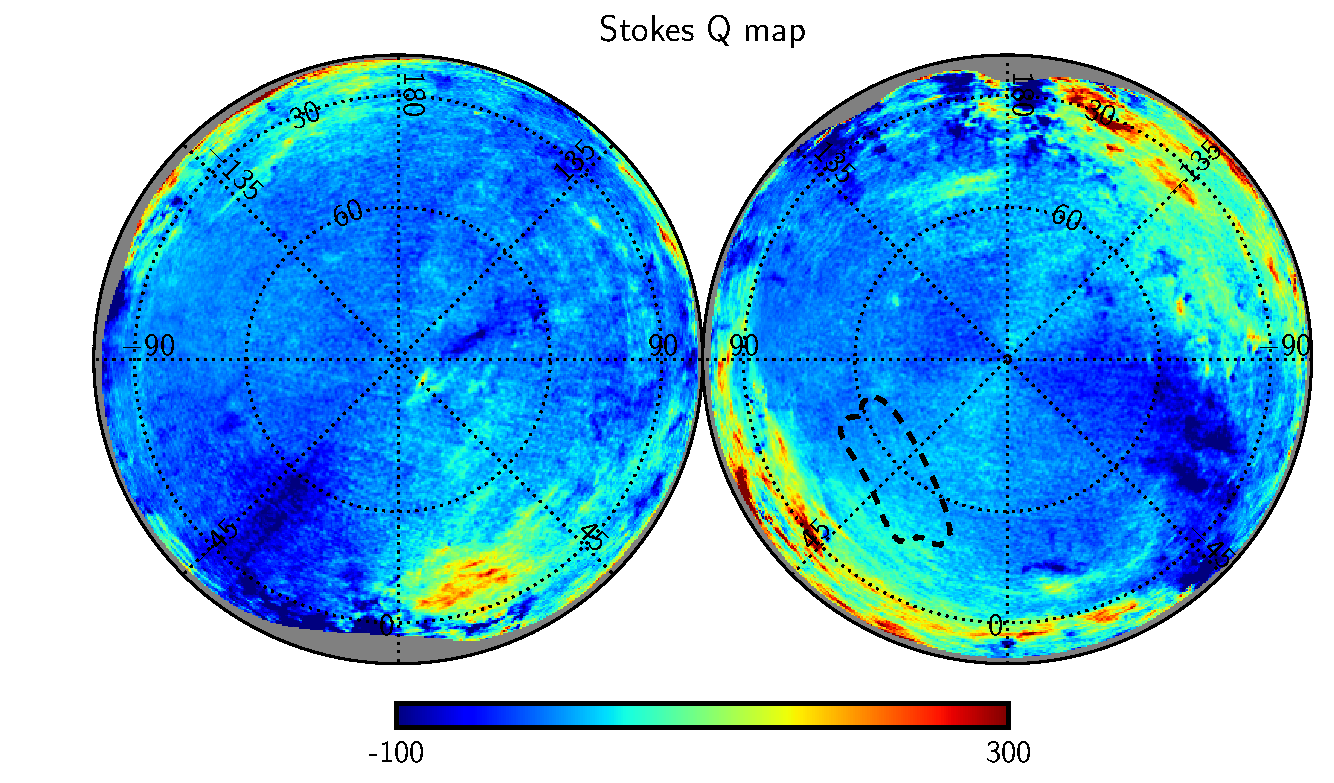
\includegraphics[width=0.47\columnwidth]{q353.pdf}}
\subfigure{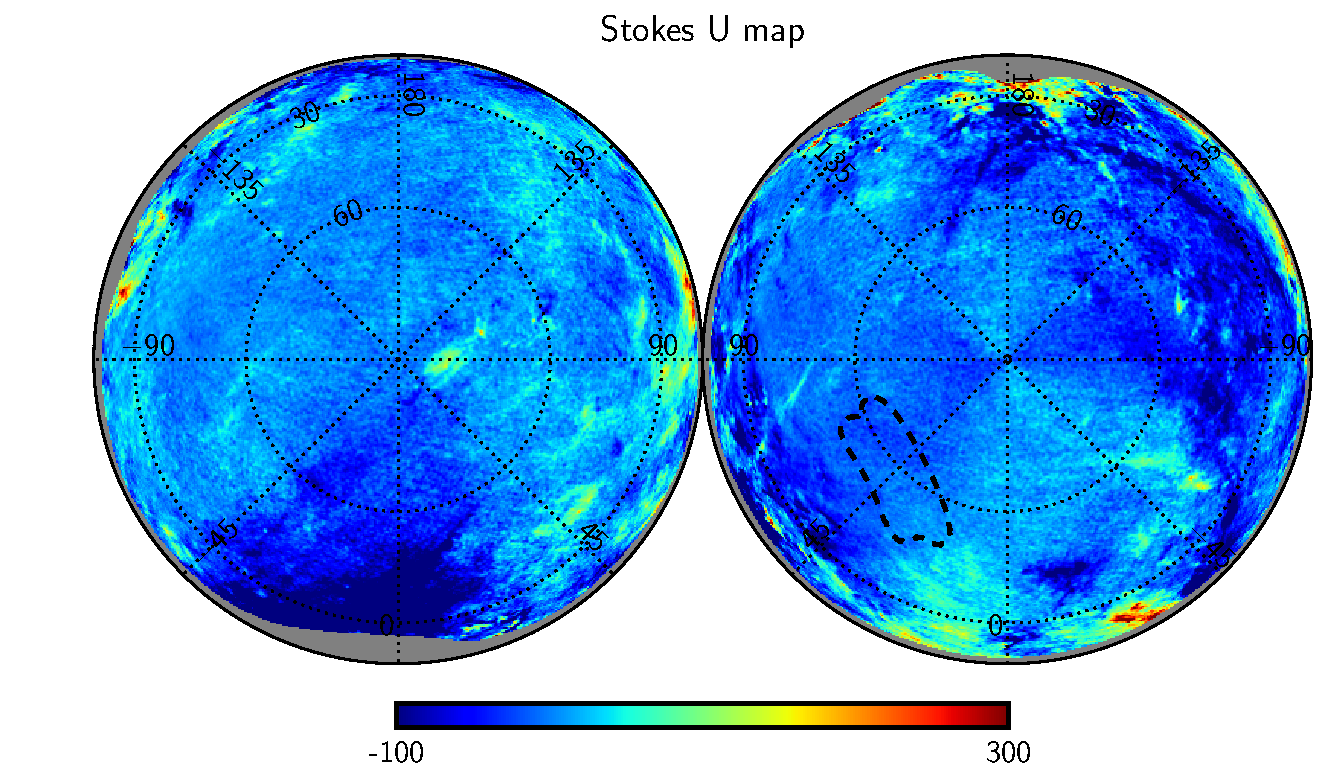
\includegraphics[width=0.47\columnwidth]{u353.pdf}}
\subfigure{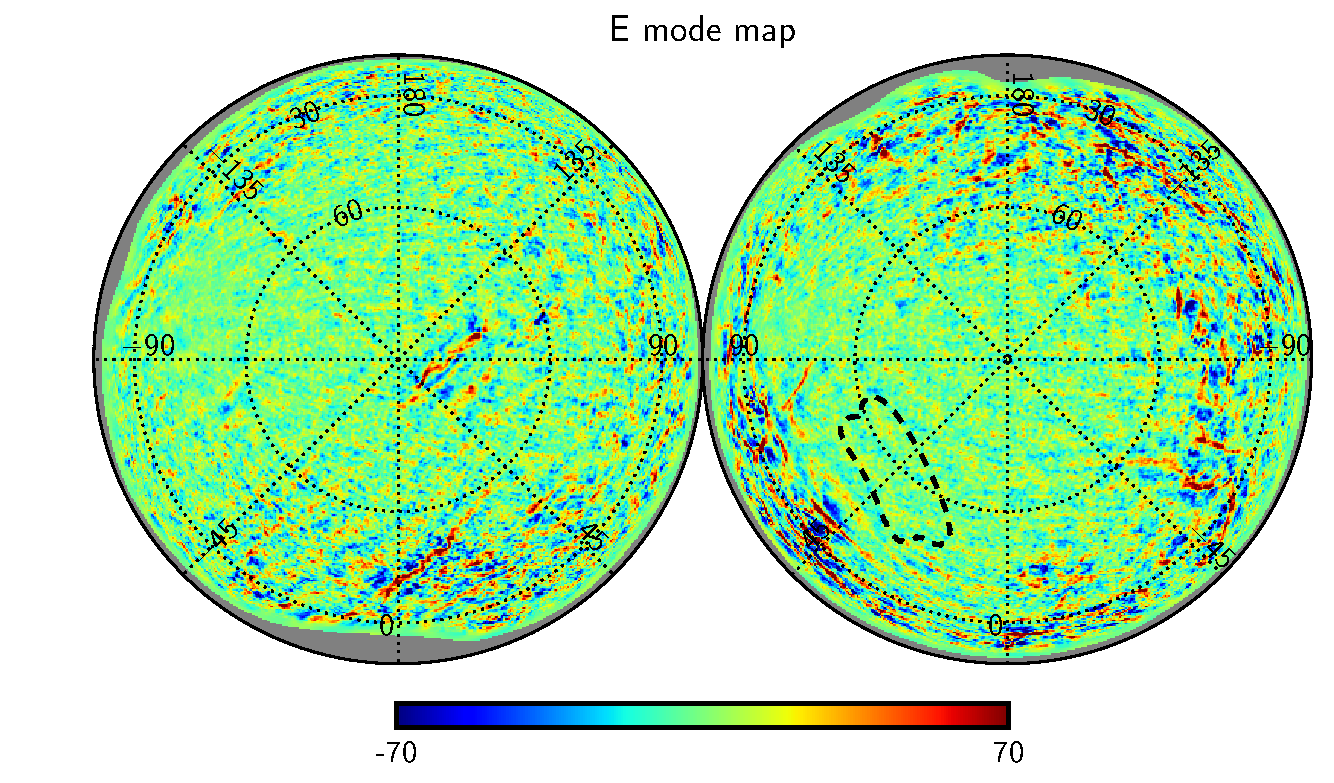
\includegraphics[width=0.47\columnwidth]{e353.pdf}}
\subfigure{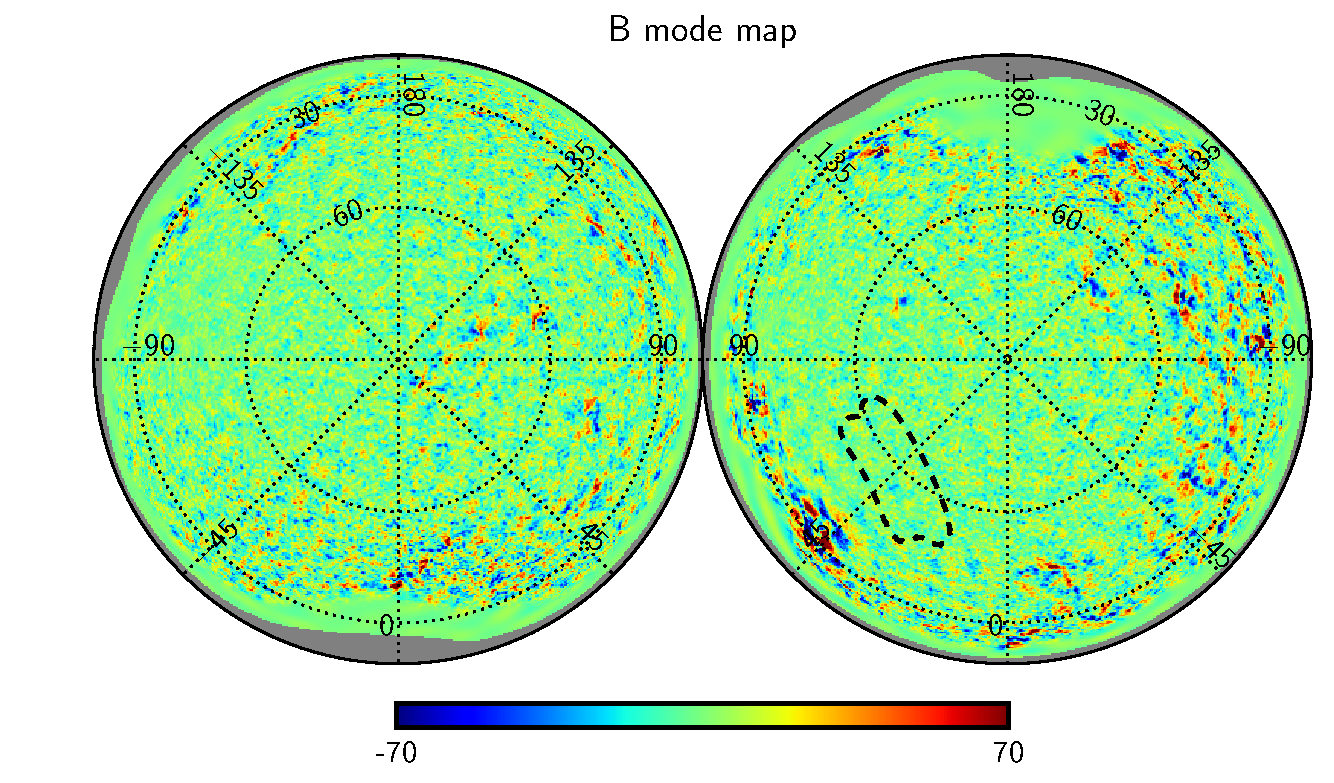
\includegraphics[width=0.47\columnwidth]{b353.pdf}}
\caption{Top left depicts the Stokes Q map while the top right depicts the Stokes U map in the 353 GHz Planck channel. The figure to the bottom left shows the E-mode map and that to the bottom right shows the B-mode maps evaluated from the Stokes paramereters. Note that while evaluating the E-mode and B-mode maps the $\ell < 40$ multipoles have been removed.}
\label{fig:ebmaps}
\end{figure}

To evaluate the local properties of polarized dust emission we closely follow the analysis presented in \cite{pip-xxx}. We sample the statistics of polarized dust emission on an Nside=8 map and only work with pixels whose galactic latitude satisfy the following criteria: $|b|>35^{\circ}$. For each pixel on the Nside=8 map satisfying this criteria, we generate a disc mask of $11.3^{\circ}$ radius with a $2^{\circ}$ apodization, centered of the coordinate of the pixel, at a resolution of Nside=512. We apply this mask on the E-mode and B-mode maps, following which we evaluate the local power spectra. We use the master algorithm to correct for the partial sky coverage. 

The error on the spectra are estimated via the following relation,
\begin{eqnarray}
\sigma_{C_{\ell}}&=&\sqrt{\frac{2}{(2\ell_{bin}+1) f_{sky} \Delta \ell}} \sqrt{C^{1}_{\ell} C^{2}_{\ell}}\,, \\
C^{1}_{\ell} C^{2}_{\ell} &=& C^{Frg}_{\ell} C^{Frg}_{\ell} + C^{Frg}_{\ell} C^{N_1}_{\ell} + C^{Frg}_{\ell} C^{N_2}_{\ell} + C^{N_1}_{\ell} C^{N_2}_{\ell}
\end{eqnarray}
where the $C_{\ell}^1$ and $C_{\ell}^2$ denote the auto-correlation power spectra derived from year-1 and year-2 measured maps. If the foreground field is to be treated as a non-stochastic field, then the relevant errors on the power spectrum should only have contribution from noise and its chance correlation with the foreground field. However the above estimate of error also includes the auto correlation power spectrum due to the foreground. In this specific sense the errors on the power spectrum are overestimated. This maybe particularly relevant to regions with strong foregrounds contribution, where the error may be dominated by the foreground power spectrum term. These regions may show up as regions with large foreground amplitudes but surprisingly low SNR assignment.

Given the power spectrum and the error estimate on it, we fit the power law spectral shapes. We carry out two separate fitting procedures,
\begin{itemize}
\item We fix the slope of the spectra ($\alpha=-2.43$) to that inferred from the global analysis. We find the best fit amplitude $[A_{sc}]$ for each region of the sky defined by the centers of pixels on a Nside=8 map.
\item We treat both the slope and the spectral amplitude as free parameters for each region of the sky. We find the best fit parameters $[A,\alpha]$ for each region of the sky defined by the centers of pixels on a Nside=8 map.
\end{itemize}
For carrying out the fitting procedure we use the in built python routine "scipy.optimize.curve\_fit", which takes the measured spectrum, the error on the spectrum and the model spectrum as input and returns the best fit parameters and the covariance for the parameters. For the case of the two parameter fit, we are currently working only with the diagonals of the covariance matrix for the parameters, in effect treating these parameters as being independent\footnote{This analysis will be refined in a future version of the analysis, where we will work with the full parameter covariance and estimate the errors from the marginalized distributions.}.

In the following analysis, we will be imposing SNR cuts to reduce the scatter dominantly driven by noise in the data. The SNR cuts imposed on $A_{sc}$ are easy to interpret, since that is the only free parameter. However while working with the two parameter fits, one needs to bear in mind the caveat that the fitted slope and the amplitude are likely to be correlated, more so in regions where the SNR is low. While searching for deviant amplitude scaling relations ($A^{BB} = 0.53 A^{EE}$)  we impose SNR cuts on $A_{sc}$. While searching for regions which deviate from the spectral slope ($\alpha=-2.43$) inferred from the global analysis, we only search in regions where $A_{sc}$ is detected at a specified SNR threshold.

\section{Statistics of amplitude and slope}

The histograms of the fitted amplitude and slope for the E and B mode spectra fitted on different portions of the sky are depicted in Fig.~\ref{fig:amp_slope_stats}. The histograms are purposefully plotted without normalization, since the heights of the histograms indicate the number of pixels which satisfy the SNR thresholds. 
\begin{figure}[!h]
\centering
\subfigure[Constant slope $(\alpha=-2.43) $]{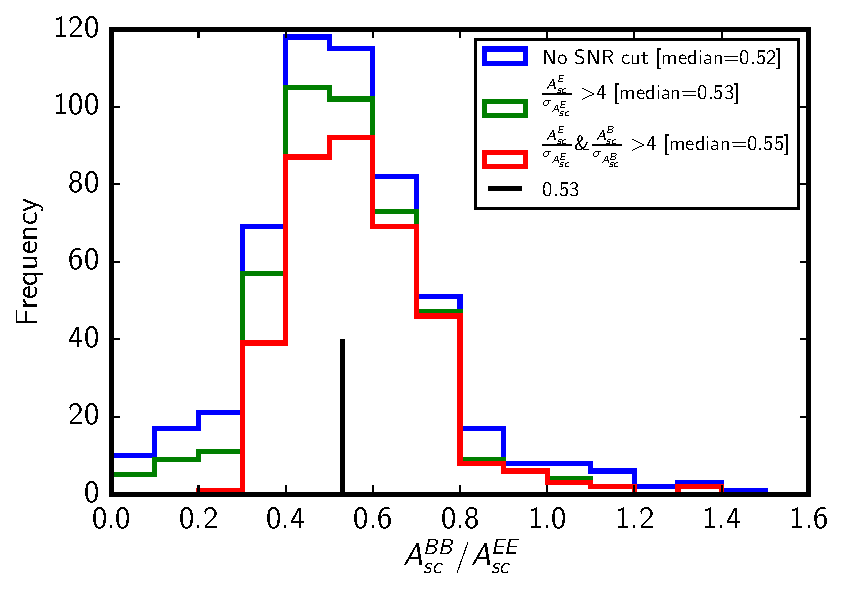
\includegraphics[width=0.3\columnwidth]{hist_amp_sc_ratio.pdf}}
\subfigure[Varying slope]{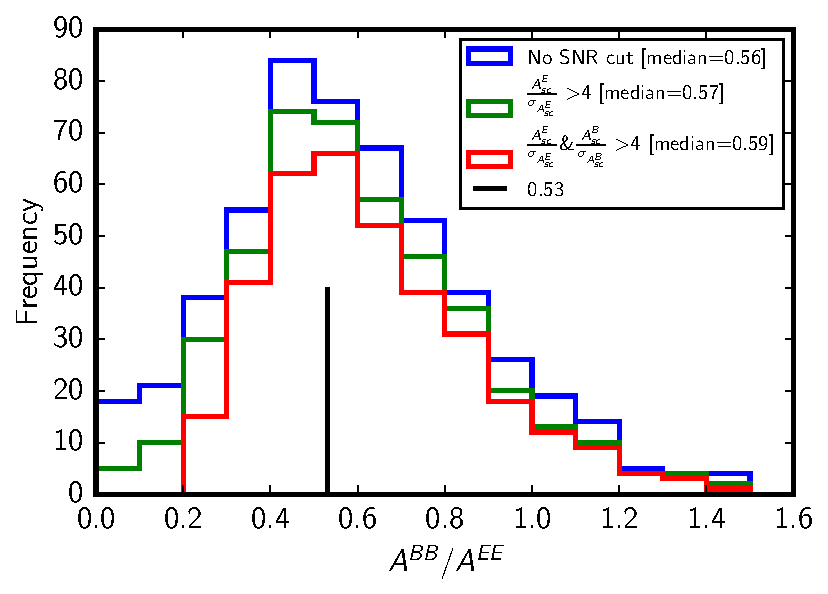
\includegraphics[width=0.3\columnwidth]{hist_amp_ratio.pdf}}
\subfigure[$\alpha$]{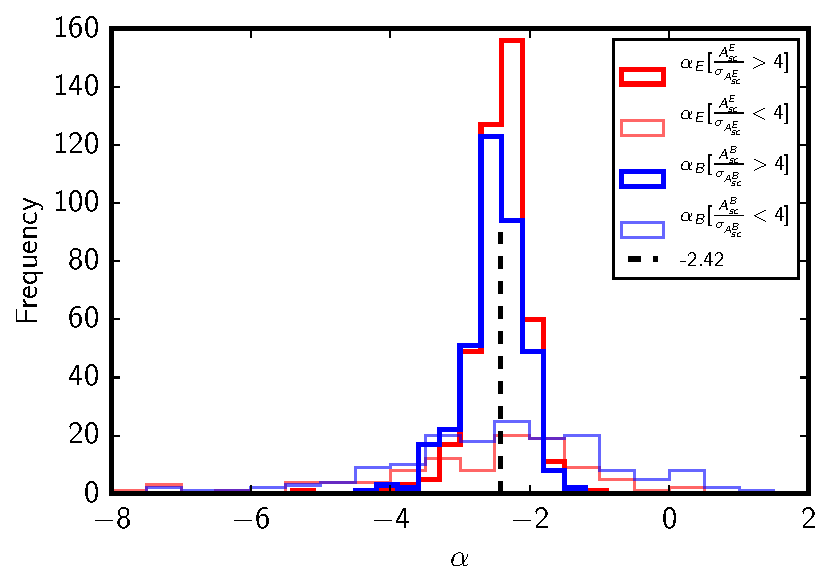
\includegraphics[width=0.3\columnwidth]{hist_spectral_slope.pdf}}
\caption{The figure on the left and in the middle depicts the histogram of ratio of B-mode amplitude to E-mode amplitude for different SNR cuts. While the figure on the left is that of amplitudes fitted for a fixed slope, the figure in the middle depicts the ratio of amplitudes when the slopes of the spectra are allowed to vary. The figure on the right depicts the histogram of fitted spectral slopes for different SNR cuts. The specifics of the SNR cuts are indicated in the figure legends.}
\label{fig:amp_slope_stats}
\end{figure}

While the histogram of amplitude ratio peaks at the empirically expected value of 0.53, it clearly shows a high end tail, indicating regions which have power in B-modes greater than expected from the empirical relation. This analysis does not reveal points where the B-mode power is much less than that expected from the empirical relation.  
 
Fig.~\ref{fig:amp_vs_ampsc} depicts the relation between $A_{sc}$ and $[A,\alpha]$. Note that $A > A_{sc}$ when the best fit slopes are steeper and $A < A_{sc}$ when the best fit slopes are shallower. 
\begin{figure}[!h]
\centering
\subfigure{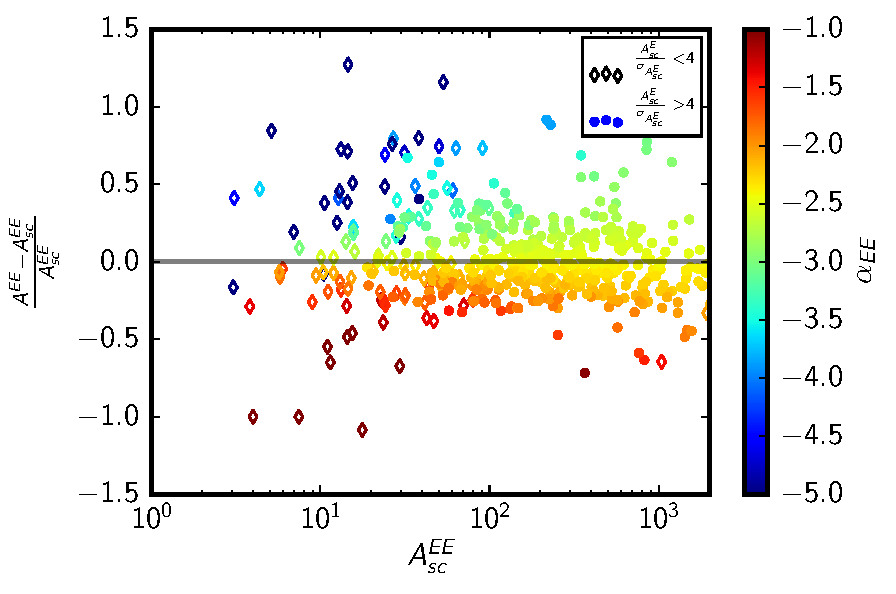
\includegraphics[width=0.47\columnwidth]{EE_amp_vsampsc.pdf}}
\subfigure{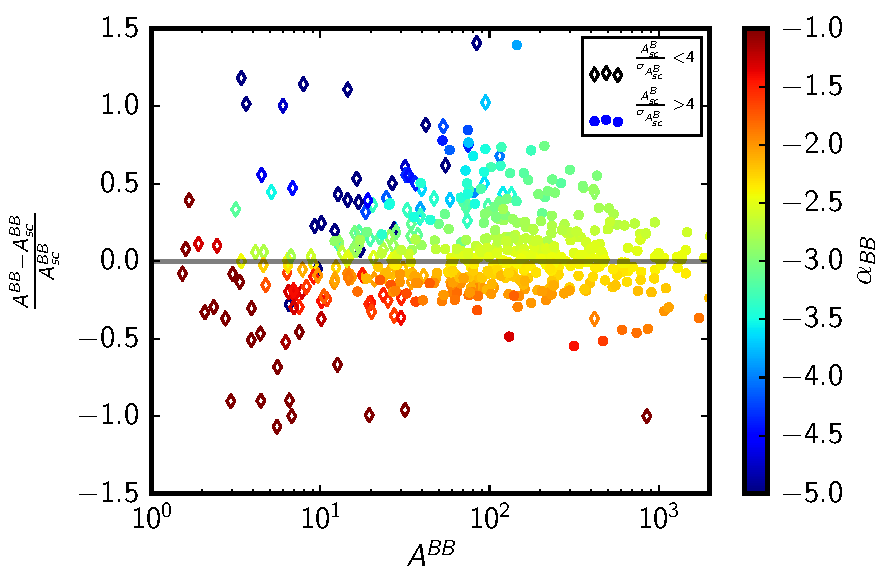
\includegraphics[width=0.47\columnwidth]{BB_amp_vsampsc.pdf}}
\caption{This figure depicts the relation between parameters $A_{sc}$ and $[A,\alpha]$ as inferred from the E-mode analysis (left) and the B-mode analysis (right). The color of the points indicate the best fit spectral slopes.}
\label{fig:amp_vs_ampsc}
\end{figure}

{\bf Comments:}
\begin{itemize}
\item Note in Fig.~\ref{fig:amp_slope_stats} that the most probable value of the ratio of amplitudes and the slopes are consistent with the global fits for amplitude and slope as indicated by the black vertical lines, in the respective plots.
\item The histogram of $A^{BB}/A^{EE}$ and $A^{BB}_{sc}/A^{EE}_{sc}$ look different in Fig.~\ref{fig:amp_slope_stats}.
\item This can be understood as arising from the definite correlation seen between the fitted amplitude and slope as seen in Fig.~\ref{fig:amp_vs_ampsc}. One needs to be careful, not to interpret Fig.~\ref{fig:amp_vs_ampsc} as an indication of varying slope in different regions of the sky, since this scatter could be potentially explained by the noise induced scatter. We will address the question of whether slope varies in different portions of the sky in a future section of this report.
\end{itemize}

\section{Are there regions of the sky which do not follow the empirical relation $A^{BB} \simeq 0.5A^{EE}$ ? }

We use the minimum distance between the point defined by the best fit  amplitudes in the pixel ``i": $[A_i^{BB},A_i^{EE}]$  and the empirical relation given by the line $A^{BB} = f A^{EE}$.
For pixels where this relation is satisfied, this distance is expected to be consistent with zero. It can be shown that the minimum distance and the error on this minimum distance is given by the following expressions,
\begin{eqnarray}
d_m &= &\frac{1}{1+f^2} (A^{BB} - fA^{EE}) ~ ; ~ \sigma^2_{d_m} = \frac{1}{1+f^2} (\sigma^2_{A^{BB}} + f^2 \sigma^2_{A^{EE})} \,,\\
{\rm SNR}&=&\frac{d_m}{\sigma_{d_m}} = \frac{A^{BB} - fA^{EE}}{\sqrt{\sigma^2_{A^{BB}} + f^2 \sigma^2_{A^{EE}}}}
\end{eqnarray}
We identify pixels for which $|{\rm SNR}| > 3.5$ as pixels which deviate from the empirical relation. Since the value of the scaling (``f") relation has a dependence on $f_{\rm sky}$, we evaluate this statistic for three different values of f and only identify pixels which are common across these range of scaling relations. The maps of pixels which show deviant behavior for different values of $f$ are shown in Fig.~\ref{fig:amp_dev_pix}
\begin{figure}[!h]
\centering
\subfigure[$f=0.45$]{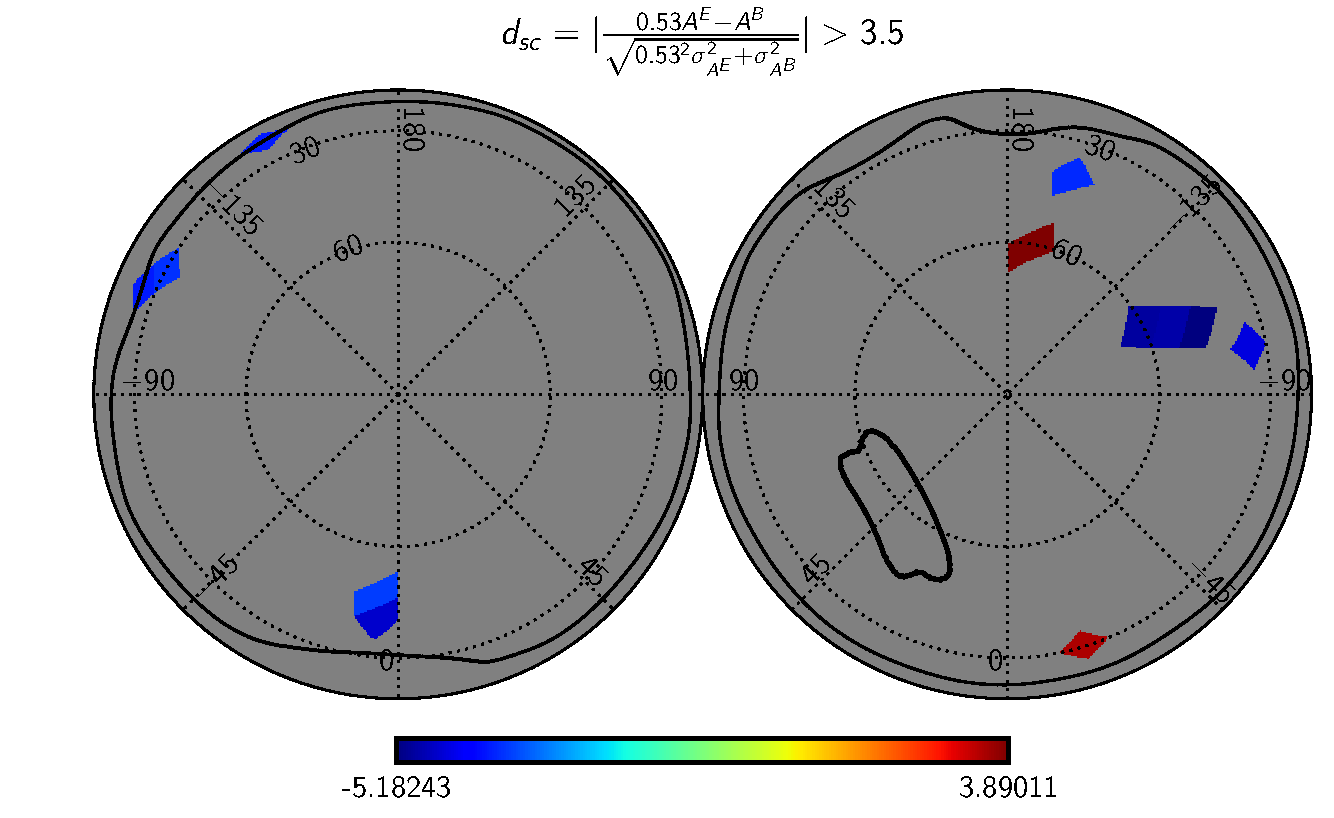
\includegraphics[width=0.32\columnwidth]{distance_bet_BE_sc_scaling53.pdf}}
\subfigure[$f=0.50$]{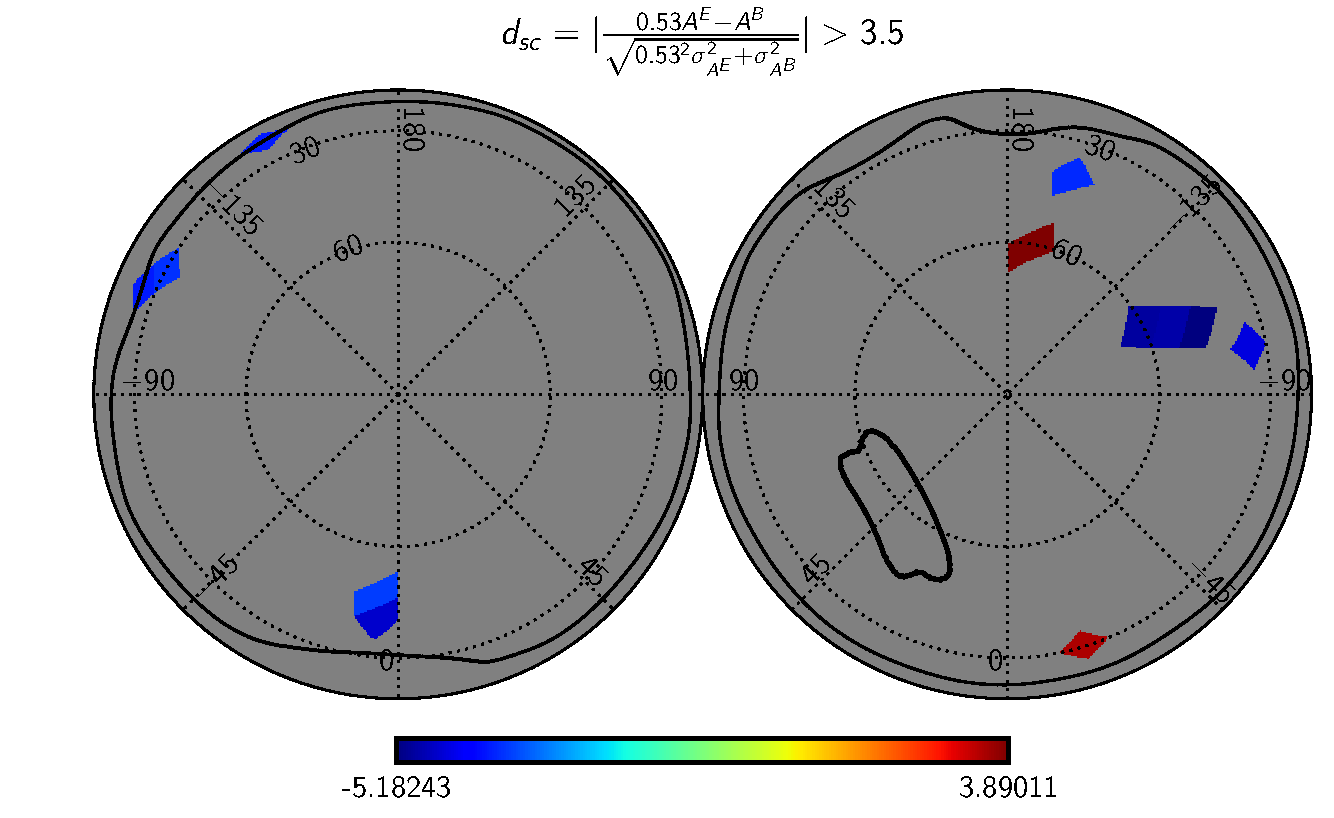
\includegraphics[width=0.32\columnwidth]{distance_bet_BE_sc_scaling53.pdf}}
\subfigure[$f=0.53$]{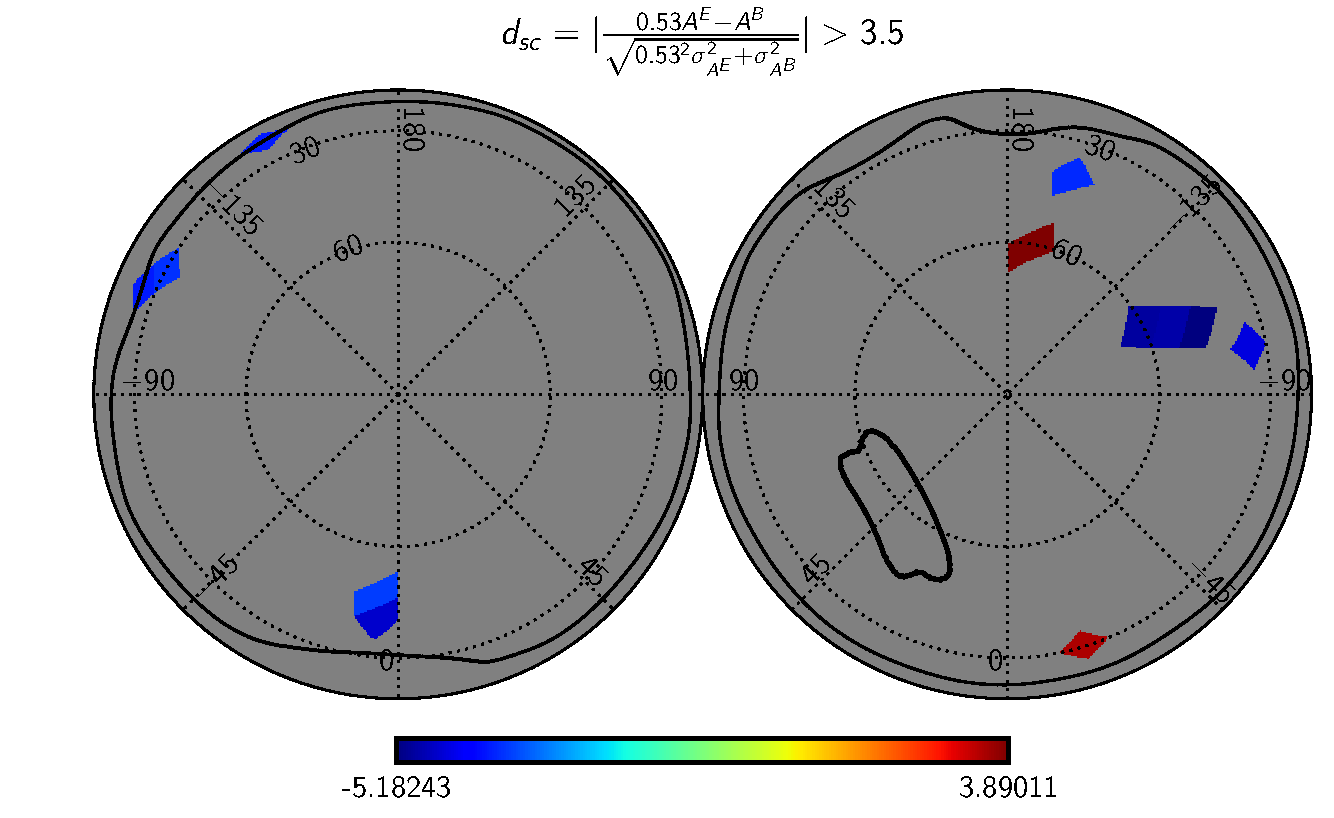
\includegraphics[width=0.32\columnwidth]{distance_bet_BE_sc_scaling53.pdf}}
\caption{The positive valued pixels coloured red are the ones for which $A^{BB} < 0.53A^{EE}$, while the negative valued pixels coloured blue are the ones for which  $A^{BB} > 0.53A^{EE}$. Note that we work with amplitudes $A_{sc}$, for which the slopes are held fixed to the global values,  while identifying these pixels.}
\label{fig:amp_dev_pix}
\end{figure}

The amplitude value and the measured slope at these deviant pixels are shown in Fig.~\ref{fig:amp_sl_scatter}.
\begin{figure}[!h]
\centering
\subfigure{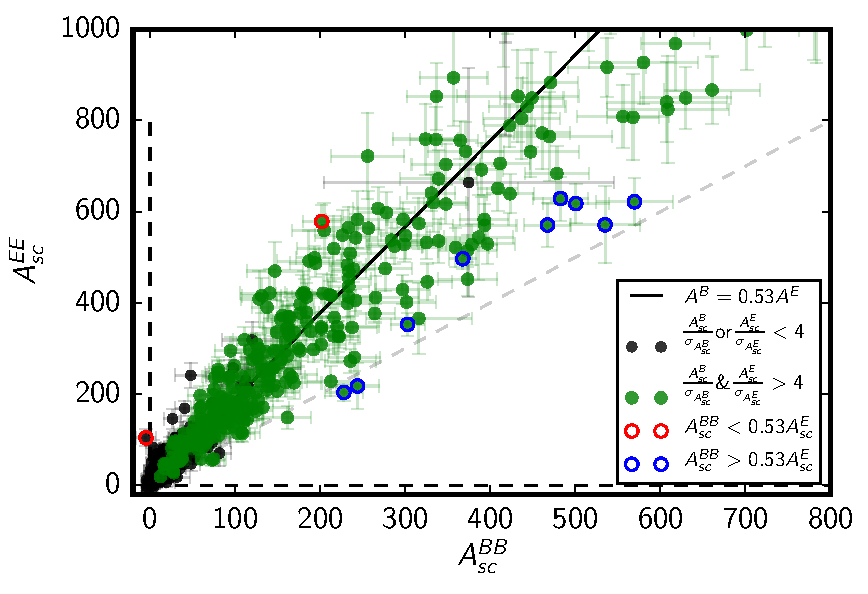
\includegraphics[width=0.47\columnwidth]{EB_amp_scatter.pdf}}
\subfigure{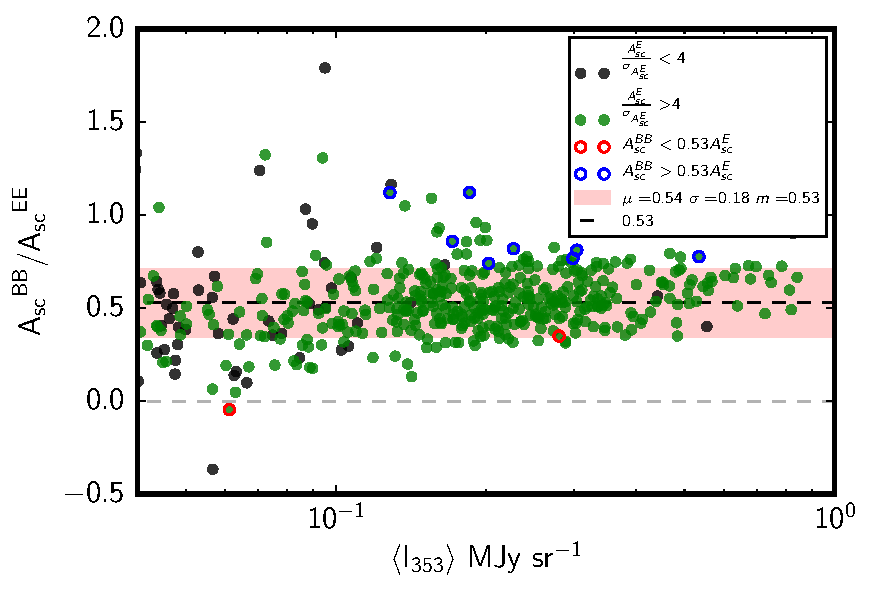
\includegraphics[width=0.47\columnwidth]{amp_ratio_vs_dustintensity.pdf}}
\subfigure{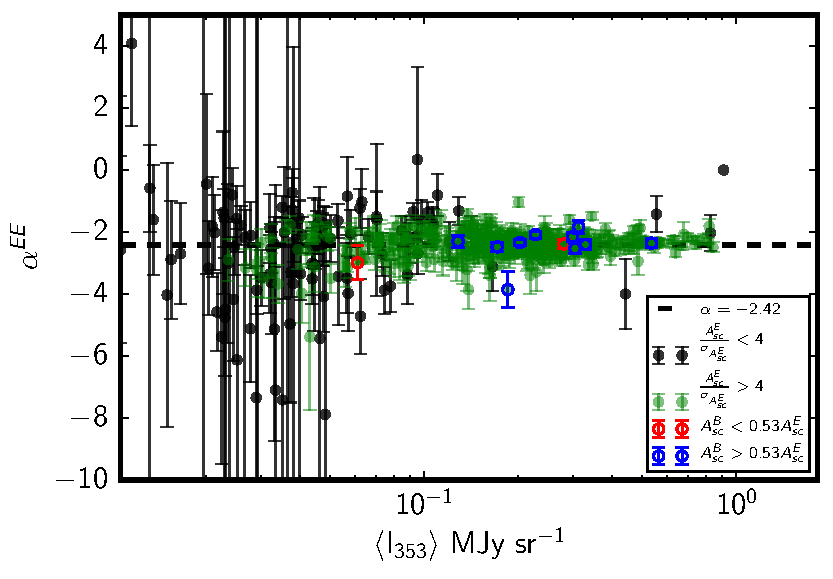
\includegraphics[width=0.47\columnwidth]{E-pol_slope_vs_dust_intensity.pdf}}
%\subfigure{\includegraphics[width=0.47\columnwidth]{B-pol_slope_vs_dust_intensity.pdf}}
\caption{Green dots depicts high SNR point which the black dots depicts the low SNR points. The red circles indicate pixels for which $A^{BB} < 0.53A^{EE}$ while the blue circles indicate pixels where $A^{BB} > 0.53A^{EE}$. {\bf Note that the slopes for the red and blue circles are consistent with the global slope.}}
\label{fig:amp_sl_scatter}
\end{figure}

The figures below depicts different tracers of the galactic foreground in regions which are found to be deviant from the global amplitude scaling relation. The maps have been centered on the respective Nside=8 pixels and masked with the disc mask hence the circular shape of the depicted regions. We have also masked using the global LR63 mask to give a more accurate depiction of the regions which contributed to the power spectra measurements. {\bf Each row in the figure below depicts the maps in a region centered on the anomalous pixel on the Nside=8 map. Zoom in on the plots to read the value of the fitted amplitudes, slopes, galactic coordinates etc. for each of the regions.}
\begin{figure}[!h]
\subfigure[T]{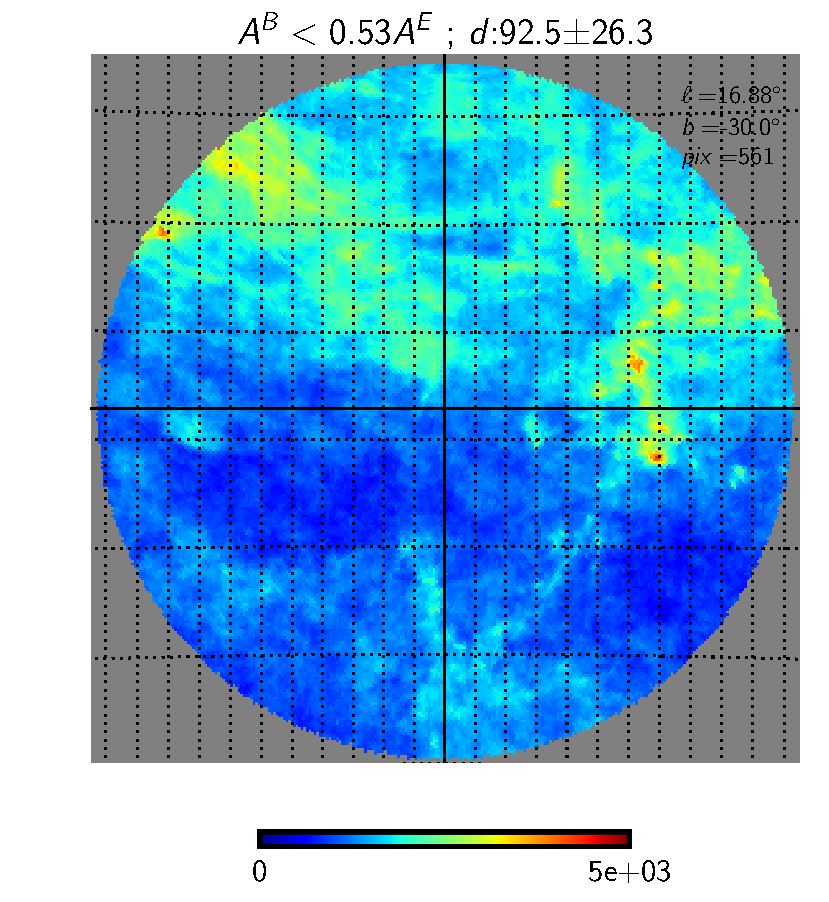
\includegraphics[width=0.1\columnwidth]{egb_scaling0.53/tmap_egb_pix561.pdf}} \hspace{-0.2cm}
\subfigure[E]{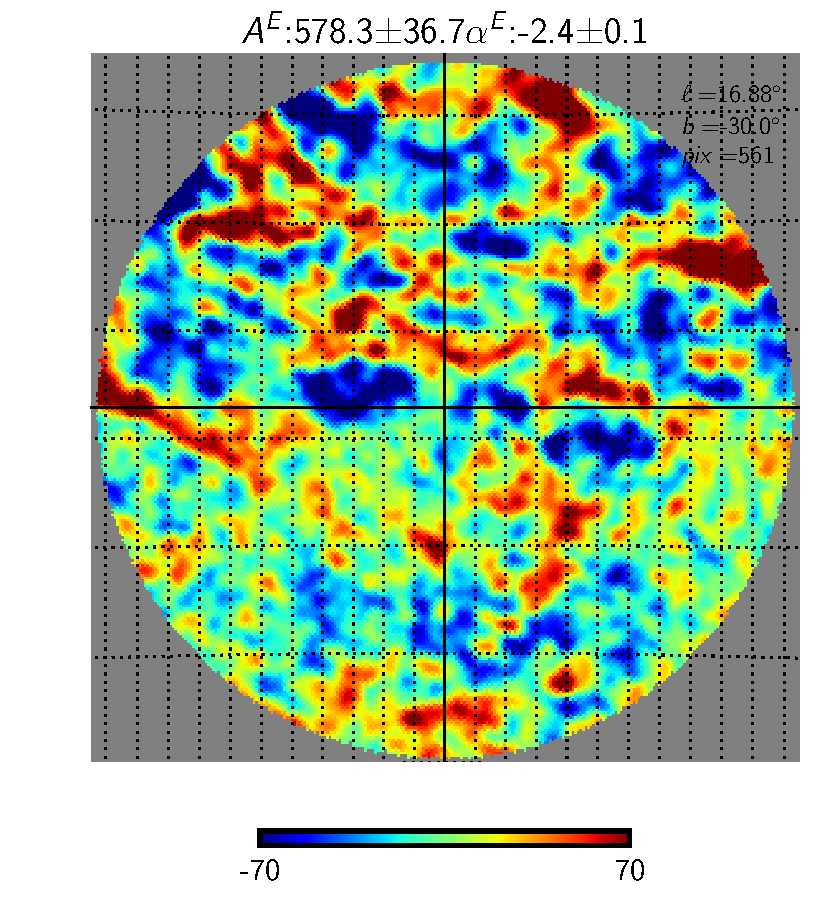
\includegraphics[width=0.1\columnwidth]{egb_scaling0.53/emap_egb_pix561.pdf}} \hspace{-0.2cm}
\subfigure[B]{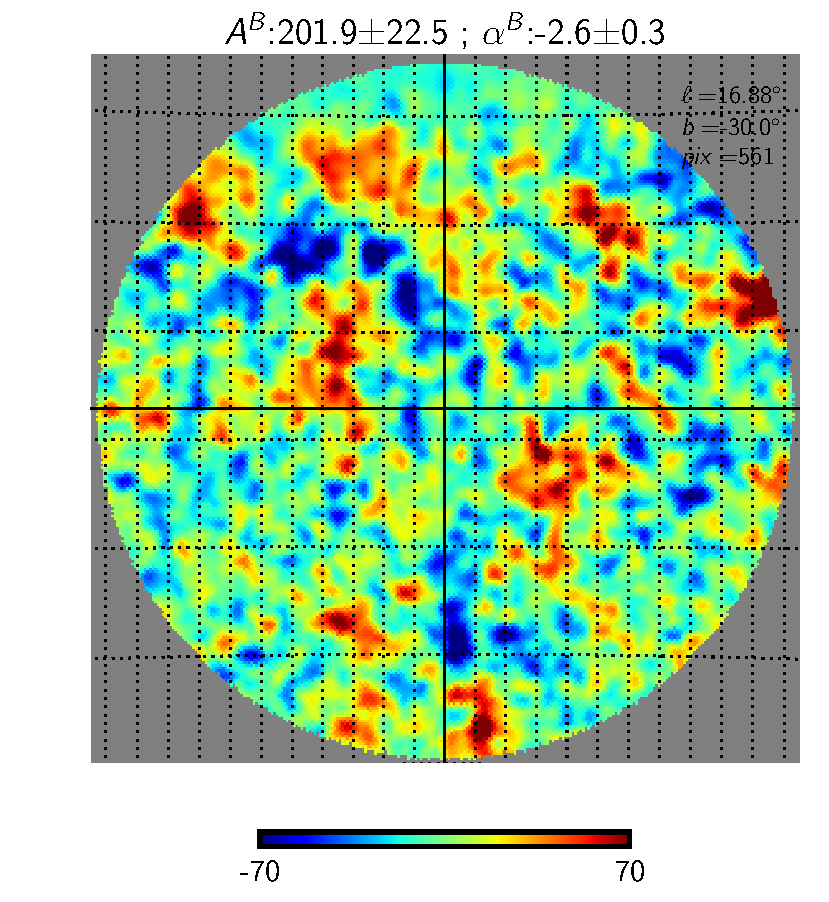
\includegraphics[width=0.1\columnwidth]{egb_scaling0.53/bmap_egb_pix561.pdf}} \hspace{-0.2cm}
\subfigure[Q]{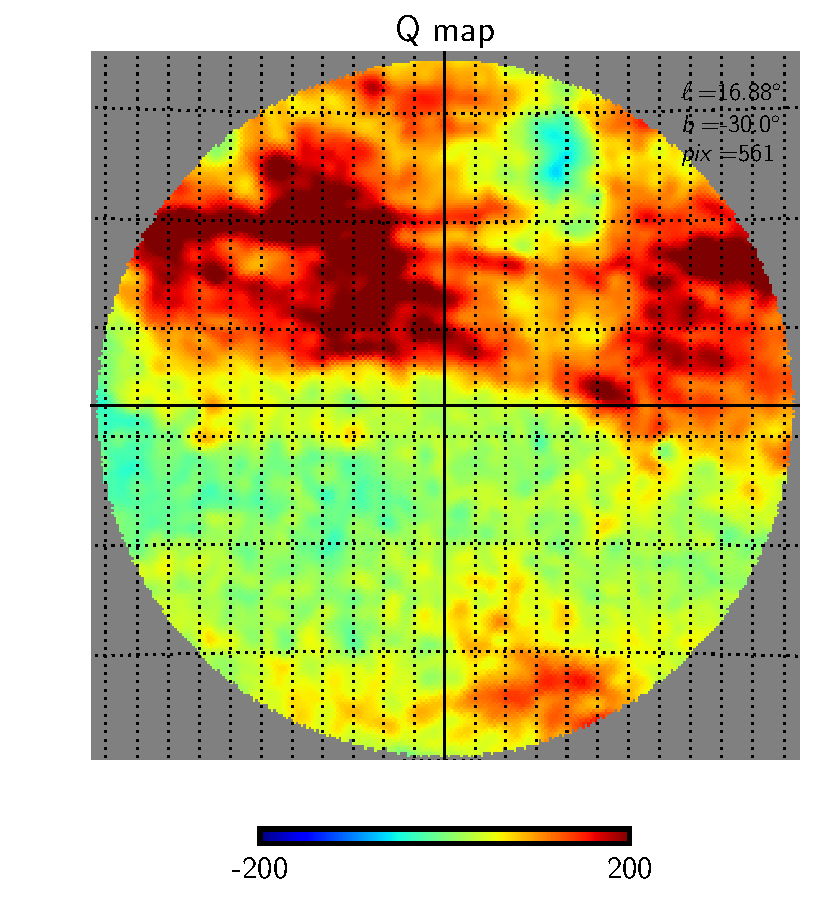
\includegraphics[width=0.1\columnwidth]{egb_scaling0.53/qmap_egb_pix561.pdf}} \hspace{-0.2cm}
\subfigure[U]{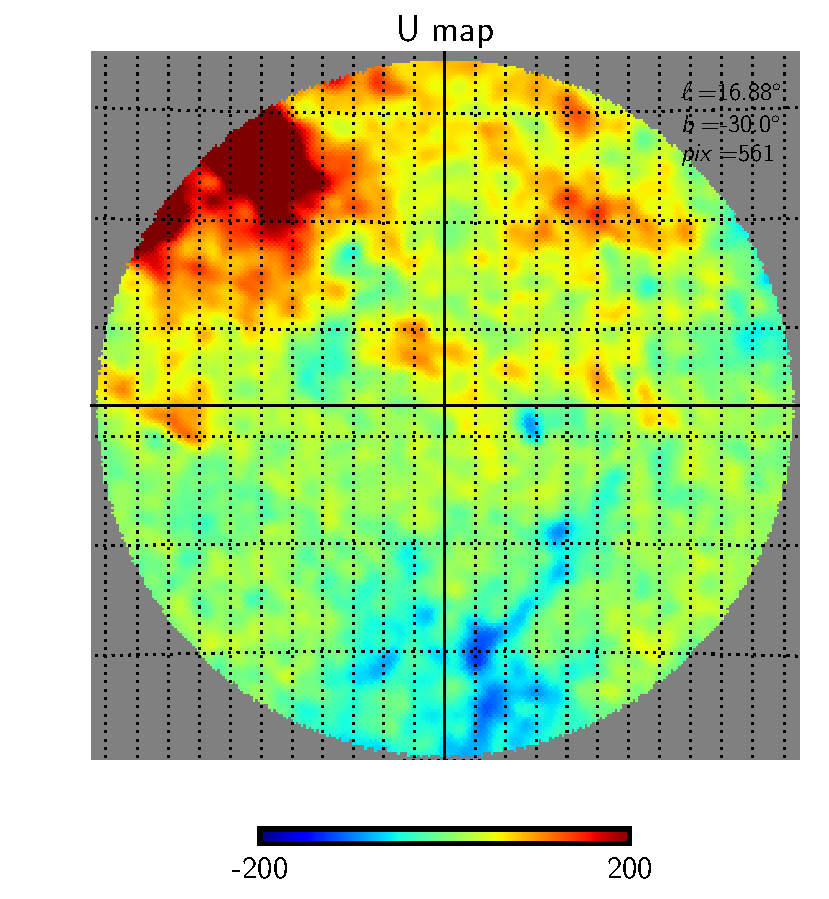
\includegraphics[width=0.1\columnwidth]{egb_scaling0.53/umap_egb_pix561.pdf}} \hspace{-0.2cm}
\subfigure[E(B-V)]{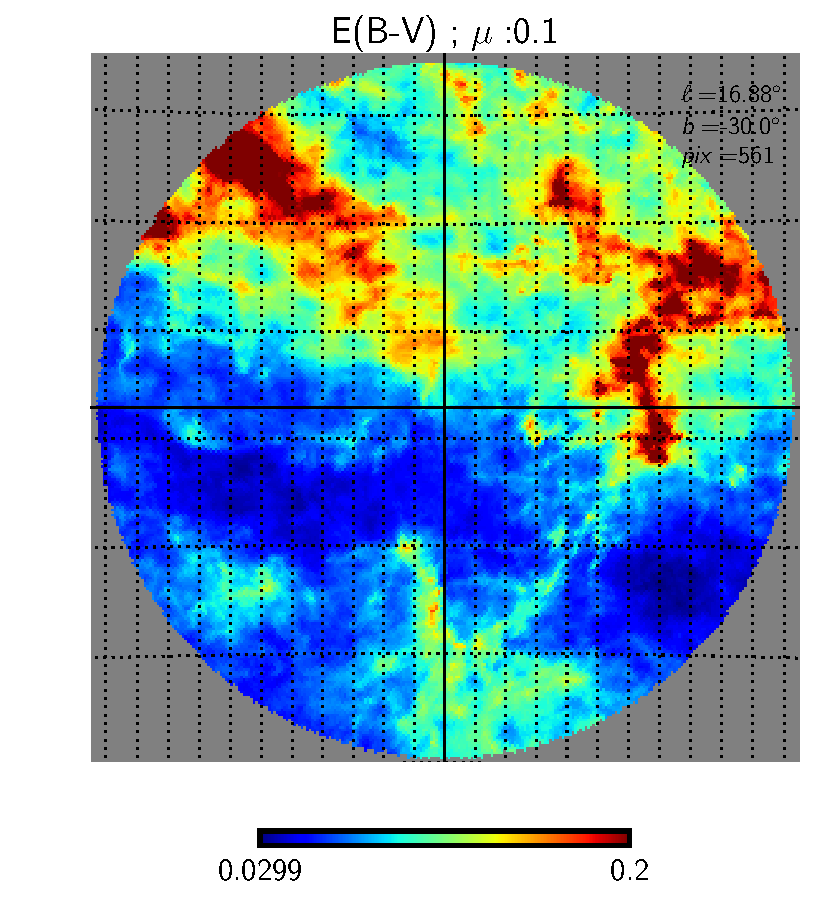
\includegraphics[width=0.1\columnwidth]{egb_scaling0.53/ebv_egb_pix561.pdf}} \hspace{-0.2cm}
\subfigure[E power]{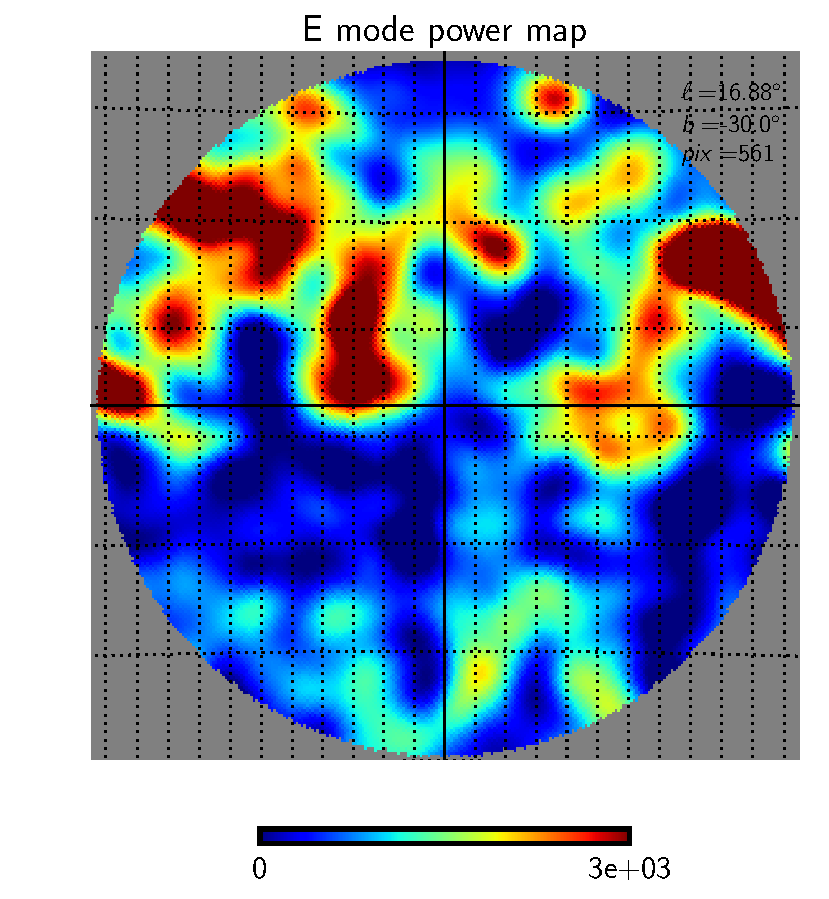
\includegraphics[width=0.1\columnwidth]{egb_scaling0.53/sqemap_egb_pix561.pdf}} \hspace{-0.2cm}
\subfigure[B power]{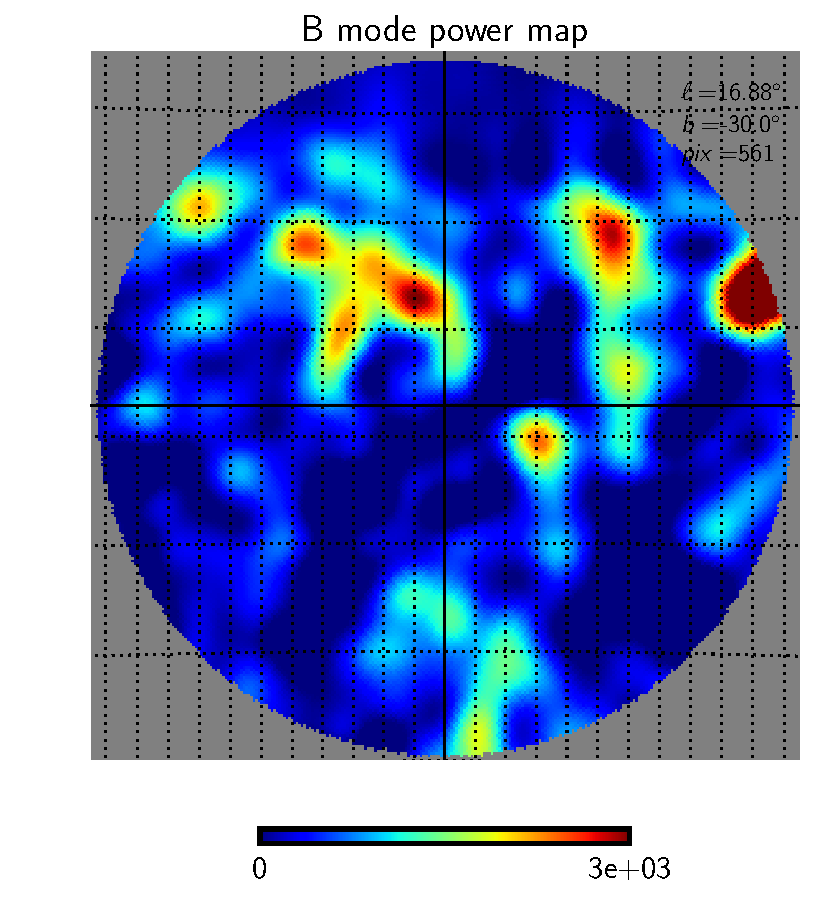
\includegraphics[width=0.1\columnwidth]{egb_scaling0.53/sqbmap_egb_pix561.pdf}} \hspace{-0.2cm}
\subfigure[NH]{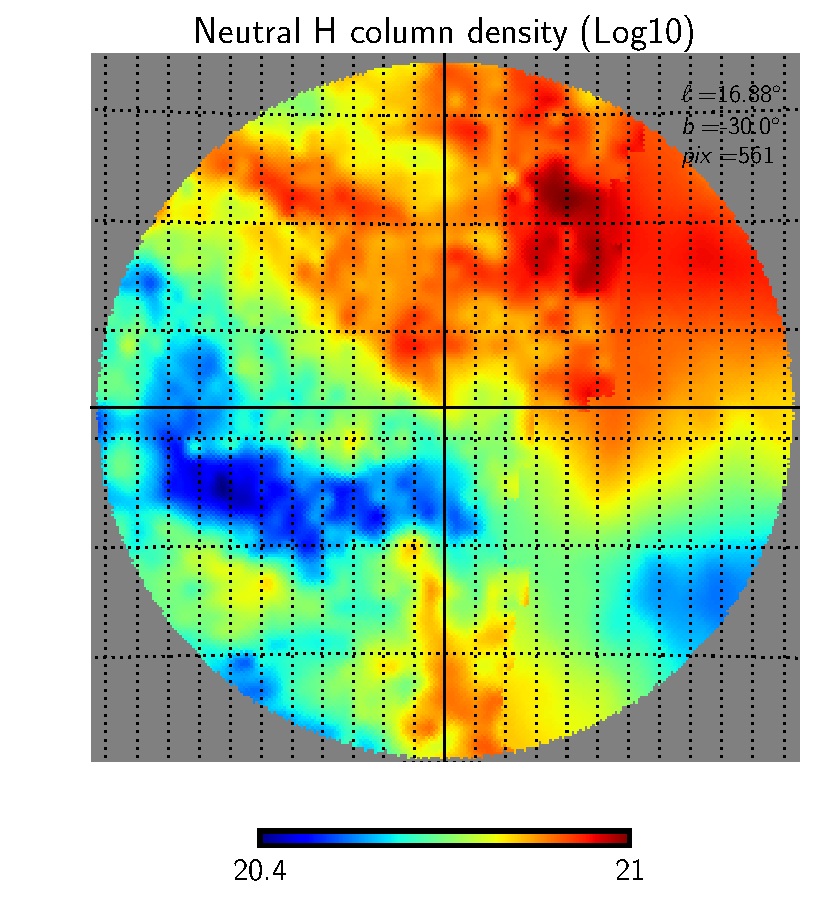
\includegraphics[width=0.1\columnwidth]{egb_scaling0.53/nhcd_egb_pix561.pdf}} \hspace{-0.2cm}
\subfigure[CO]{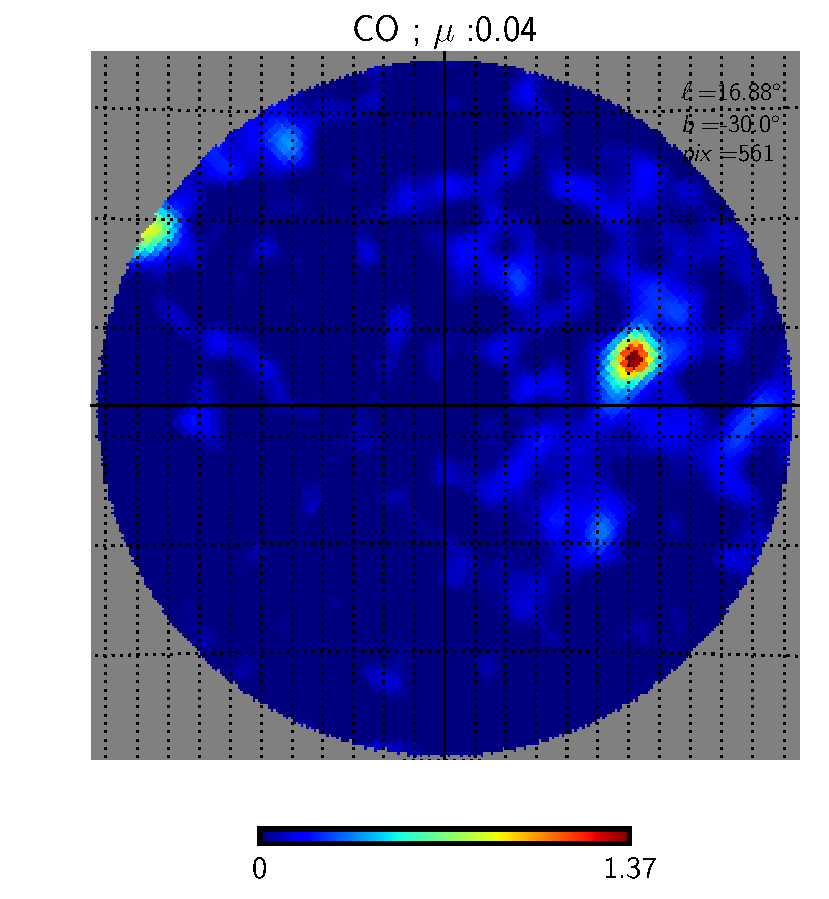
\includegraphics[width=0.1\columnwidth]{egb_scaling0.53/co_egb_pix561.pdf}} \hspace{-0.2cm}
%\subfigure{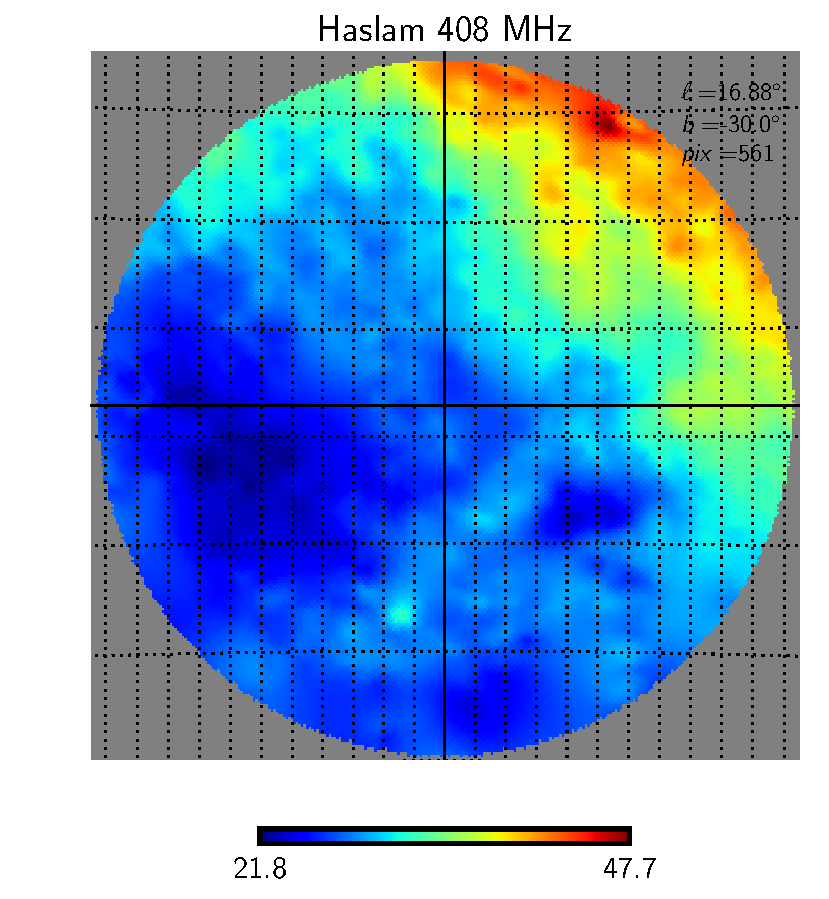
\includegraphics[width=0.1\columnwidth]{egb_scaling0.53/haslam_egb_pix561.pdf}} \hspace{-0.2cm}
%\end{figure}
%\begin{figure}[!h]
\subfigure {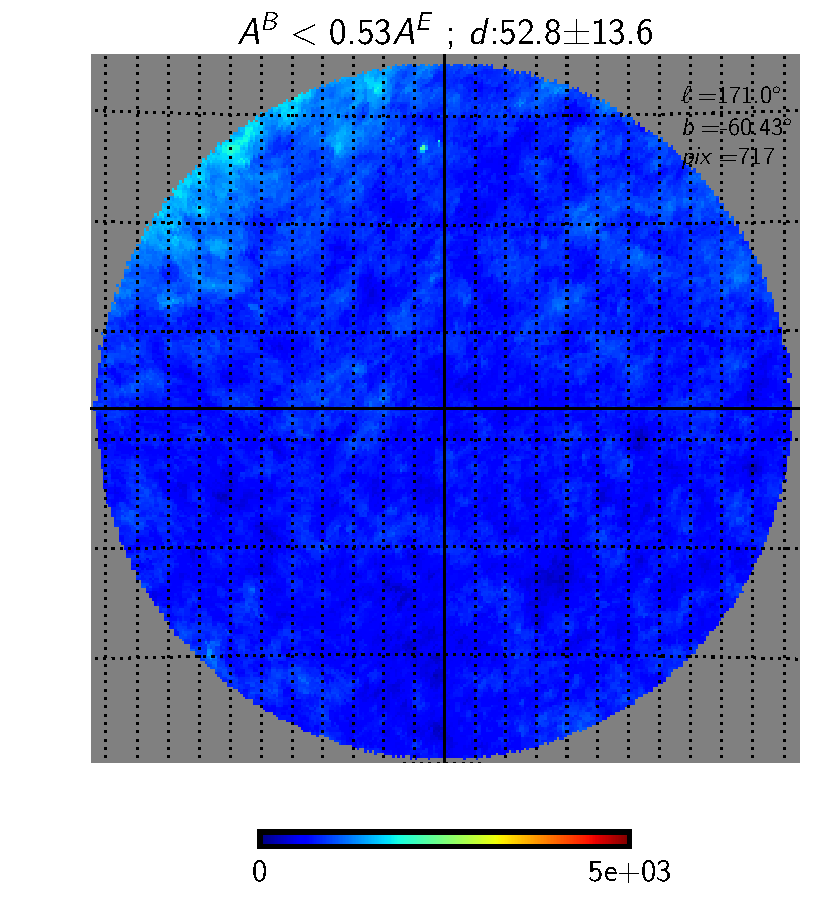
\includegraphics[width=0.1\columnwidth]{egb_scaling0.53/tmap_egb_pix717.pdf}} \hspace{-0.2cm}
\subfigure{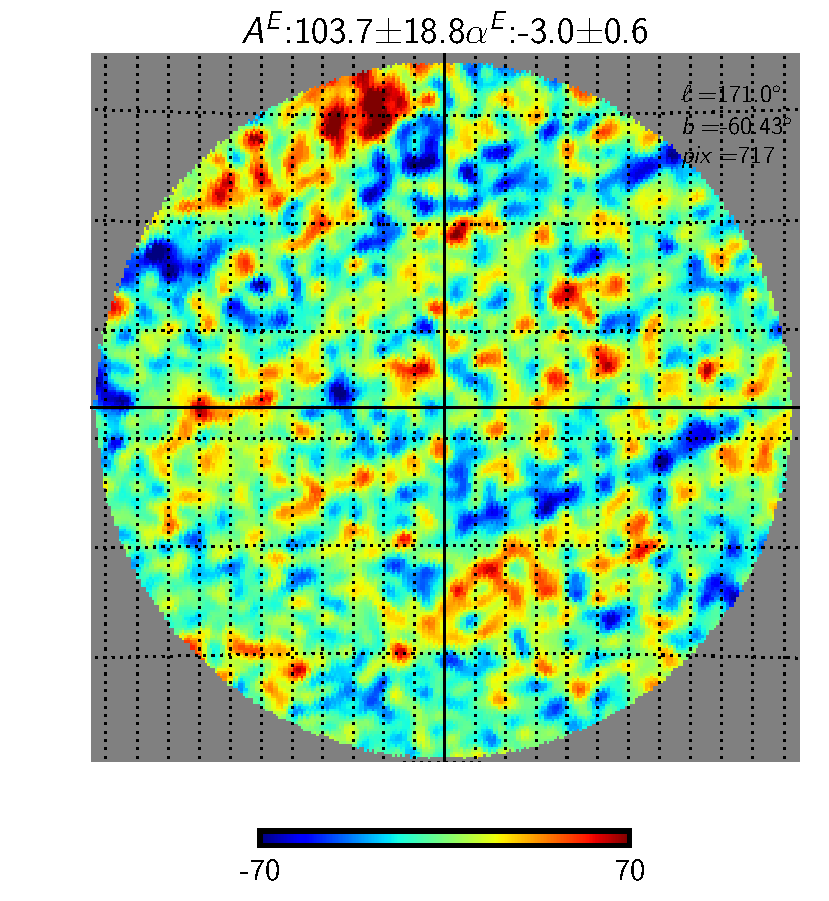
\includegraphics[width=0.1\columnwidth]{egb_scaling0.53/emap_egb_pix717.pdf}} \hspace{-0.2cm}
\subfigure{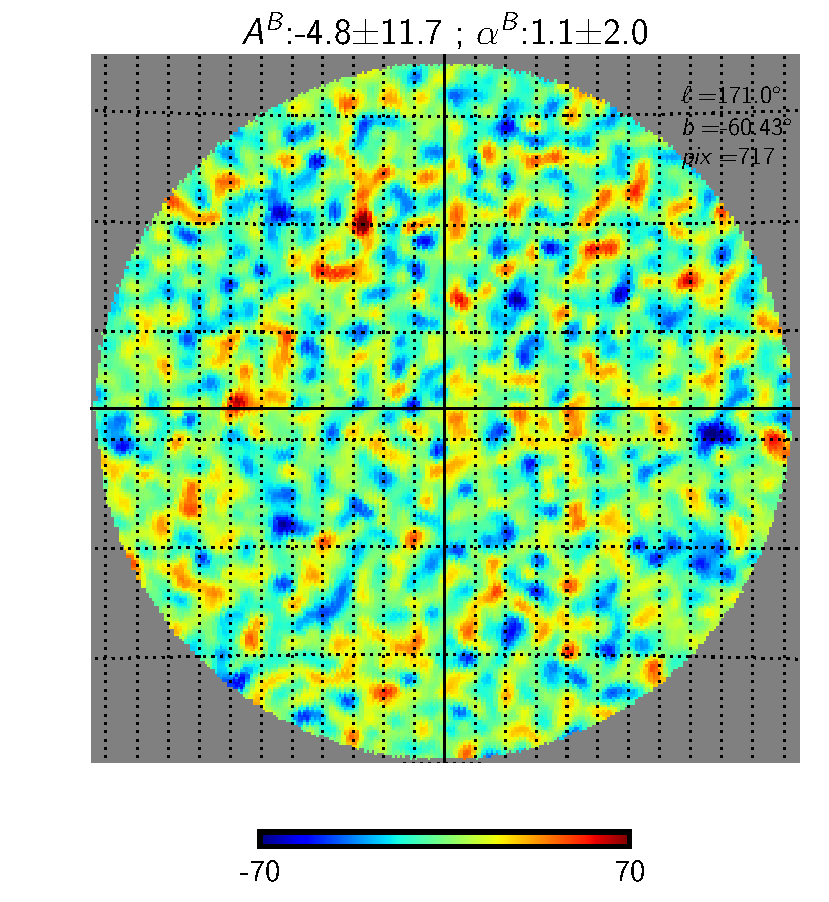
\includegraphics[width=0.1\columnwidth]{egb_scaling0.53/bmap_egb_pix717.pdf}} \hspace{-0.2cm}
\subfigure{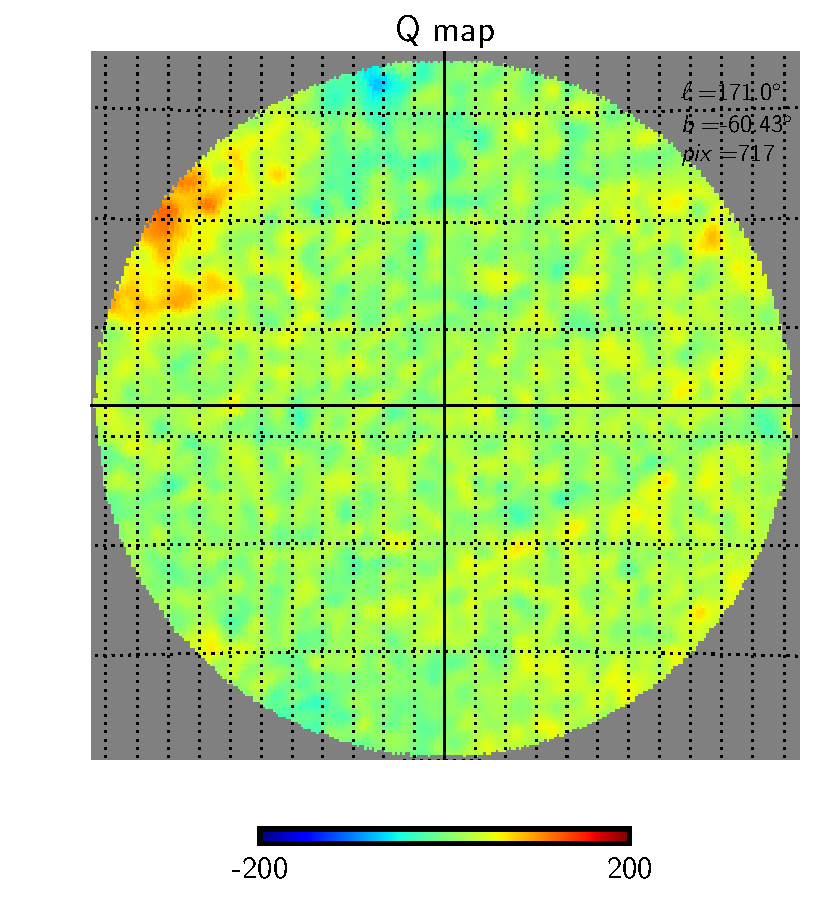
\includegraphics[width=0.1\columnwidth]{egb_scaling0.53/qmap_egb_pix717.pdf}} \hspace{-0.2cm}
\subfigure{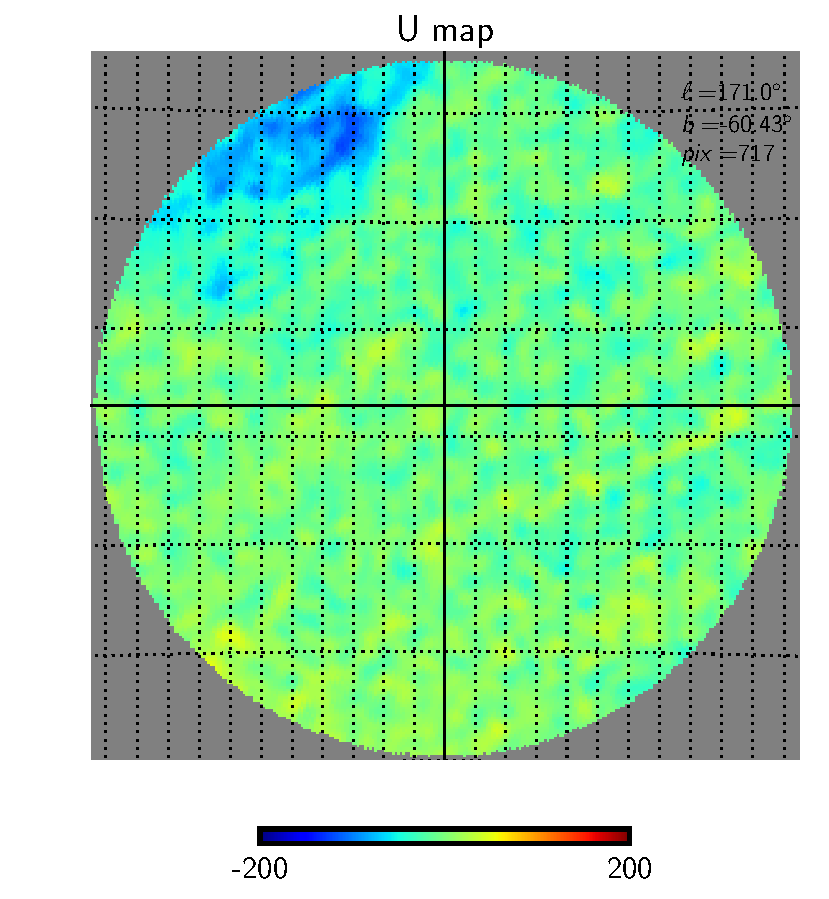
\includegraphics[width=0.1\columnwidth]{egb_scaling0.53/umap_egb_pix717.pdf}} \hspace{-0.2cm}
\subfigure{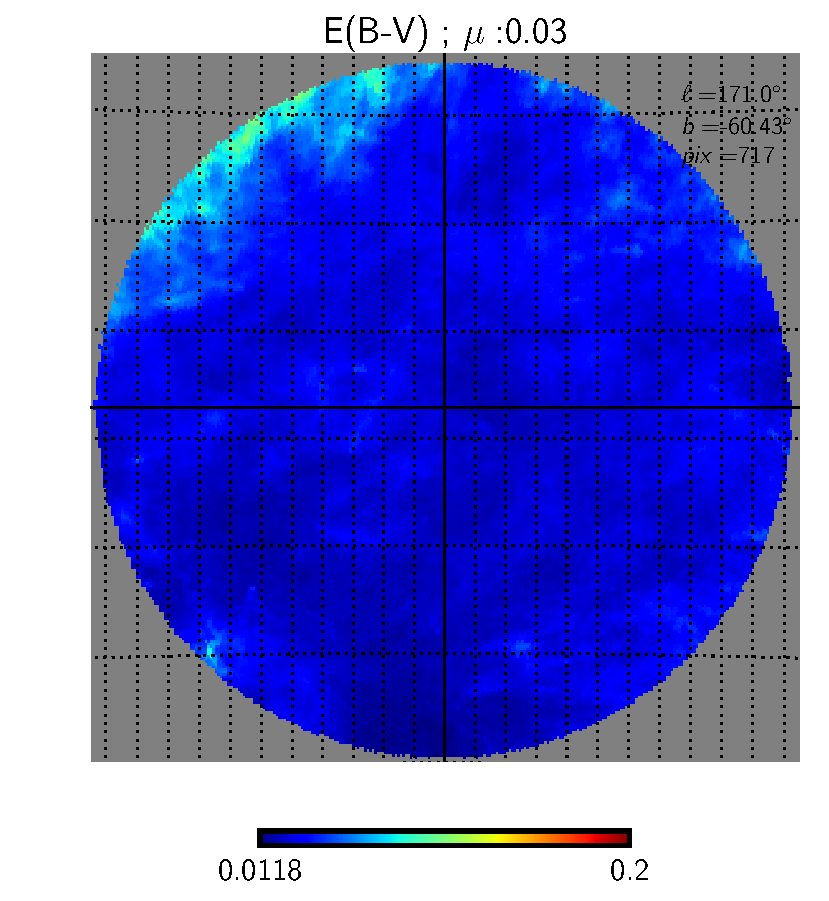
\includegraphics[width=0.1\columnwidth]{egb_scaling0.53/ebv_egb_pix717.pdf}} \hspace{-0.2cm}
\subfigure{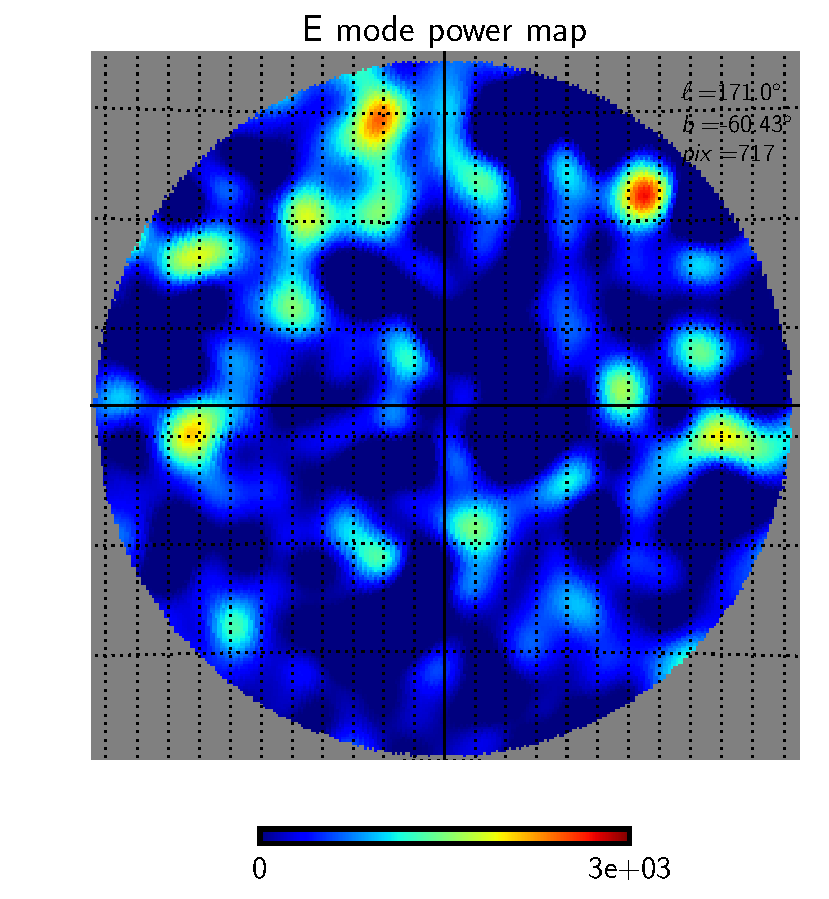
\includegraphics[width=0.1\columnwidth]{egb_scaling0.53/sqemap_egb_pix717.pdf}} \hspace{-0.2cm}
\subfigure{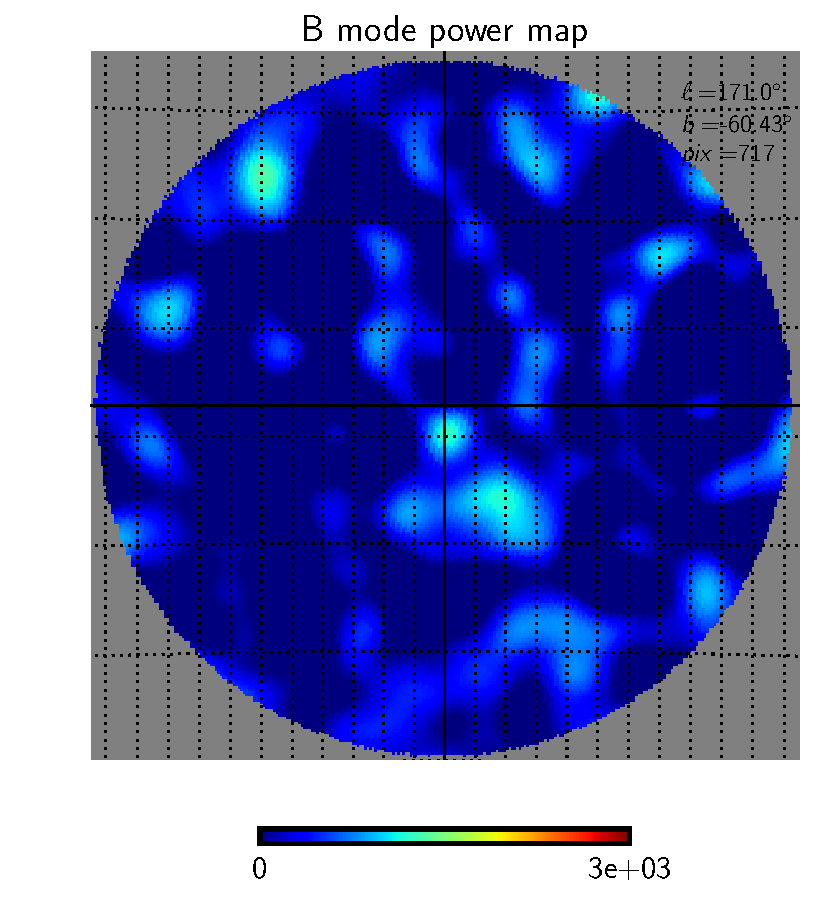
\includegraphics[width=0.1\columnwidth]{egb_scaling0.53/sqbmap_egb_pix717.pdf}} \hspace{-0.2cm}
\subfigure{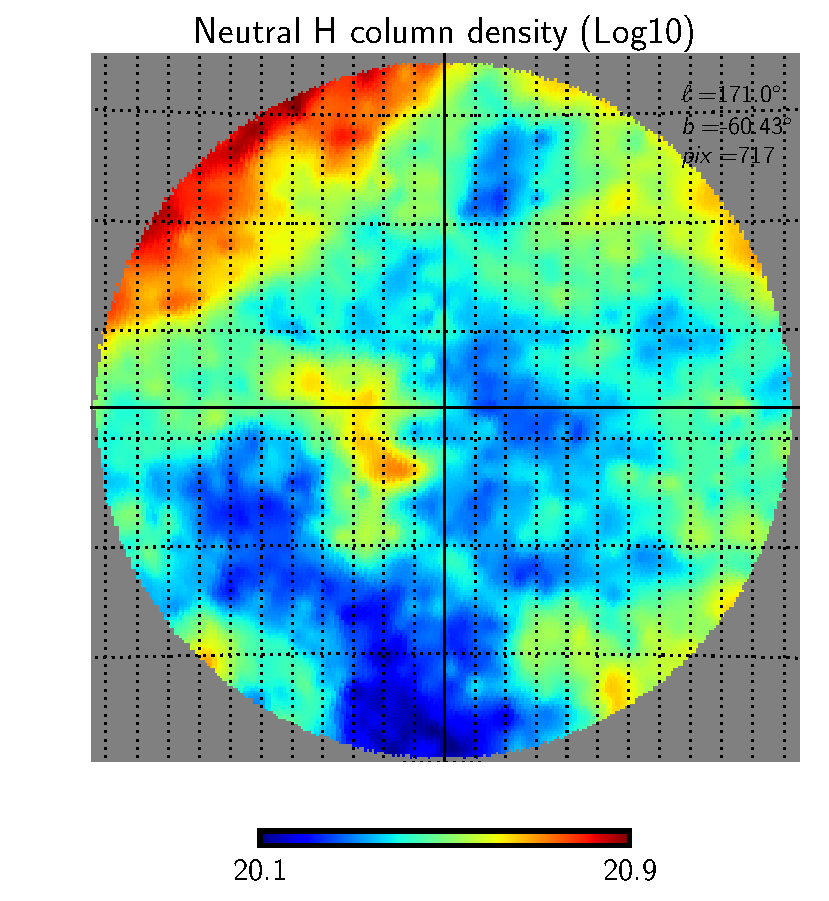
\includegraphics[width=0.1\columnwidth]{egb_scaling0.53/nhcd_egb_pix717.pdf}} \hspace{-0.2cm}
\subfigure{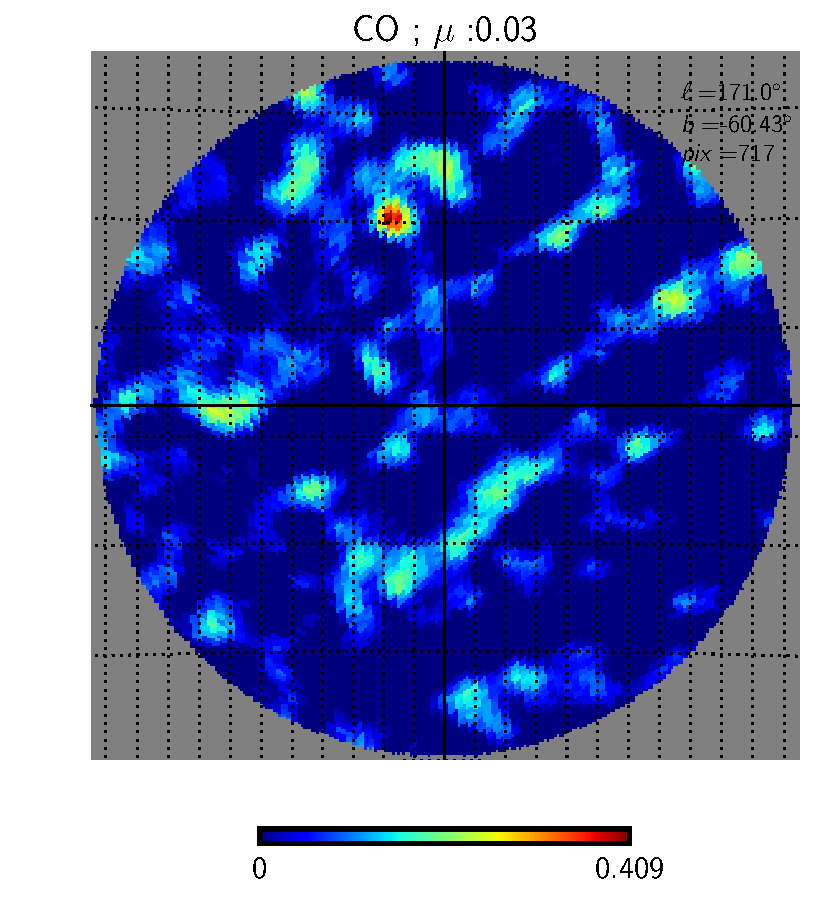
\includegraphics[width=0.1\columnwidth]{egb_scaling0.53/co_egb_pix717.pdf}} \hspace{-0.2cm}
%\subfigure{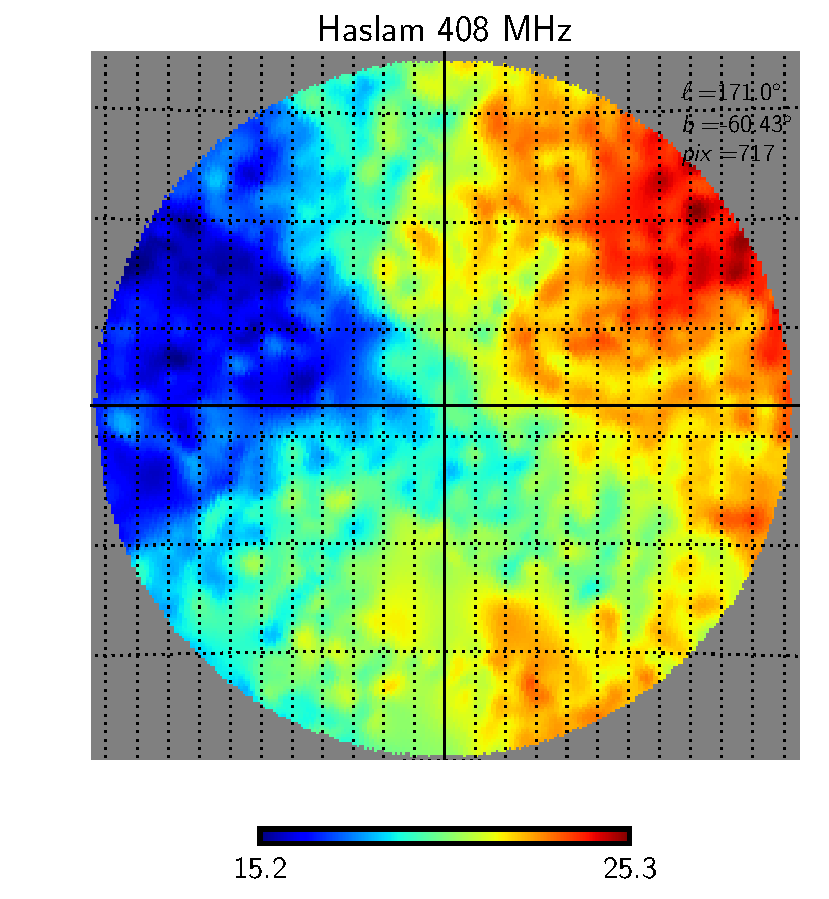
\includegraphics[width=0.1\columnwidth]{egb_scaling0.53/haslam_egb_pix717.pdf}} \hspace{-0.2cm}
\caption{\color{red}{$A^{BB}_{sc} < f A^{EE}_{sc}$}}
\end{figure}

\begin{figure}[!h]
\subfigure[T]{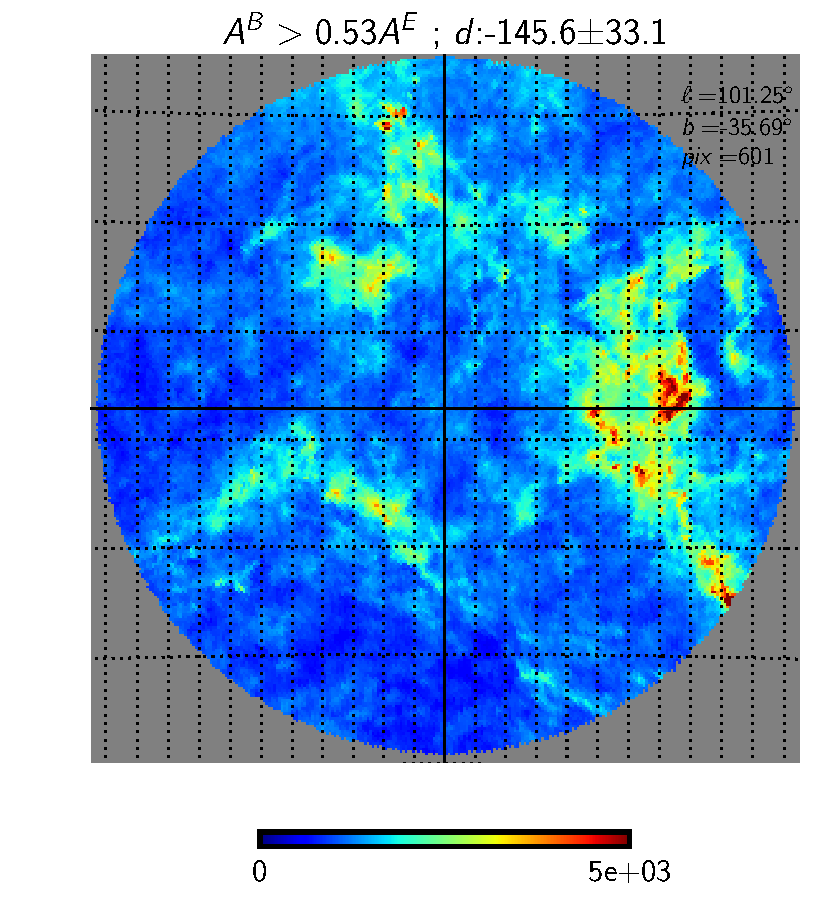
\includegraphics[width=0.1\columnwidth]{bge_scaling0.53/tmap_bge_pix601.pdf}} \hspace{-0.2cm}
\subfigure[E]{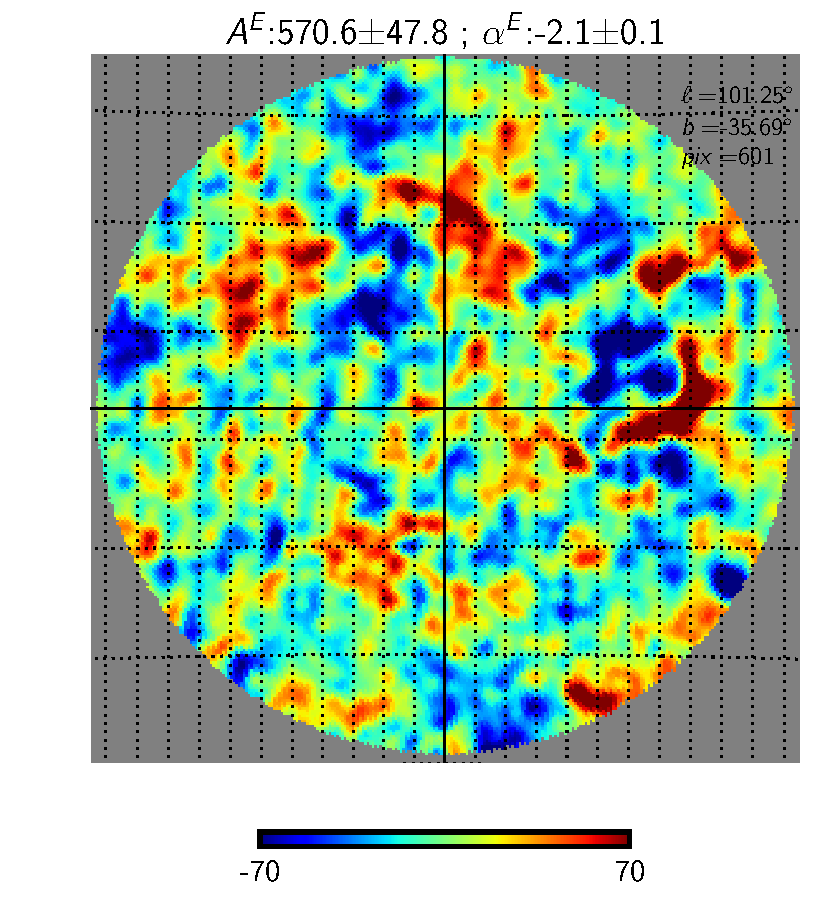
\includegraphics[width=0.1\columnwidth]{bge_scaling0.53/emap_bge_pix601.pdf}} \hspace{-0.2cm}
\subfigure[B]{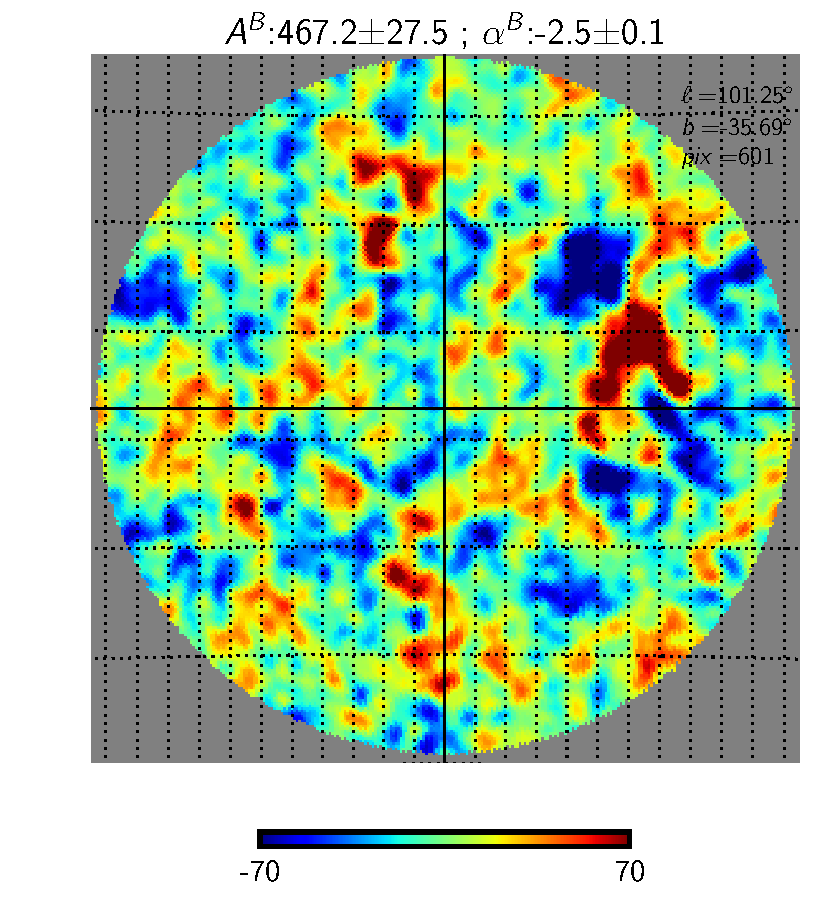
\includegraphics[width=0.1\columnwidth]{bge_scaling0.53/bmap_bge_pix601.pdf}} \hspace{-0.2cm}
\subfigure[Q]{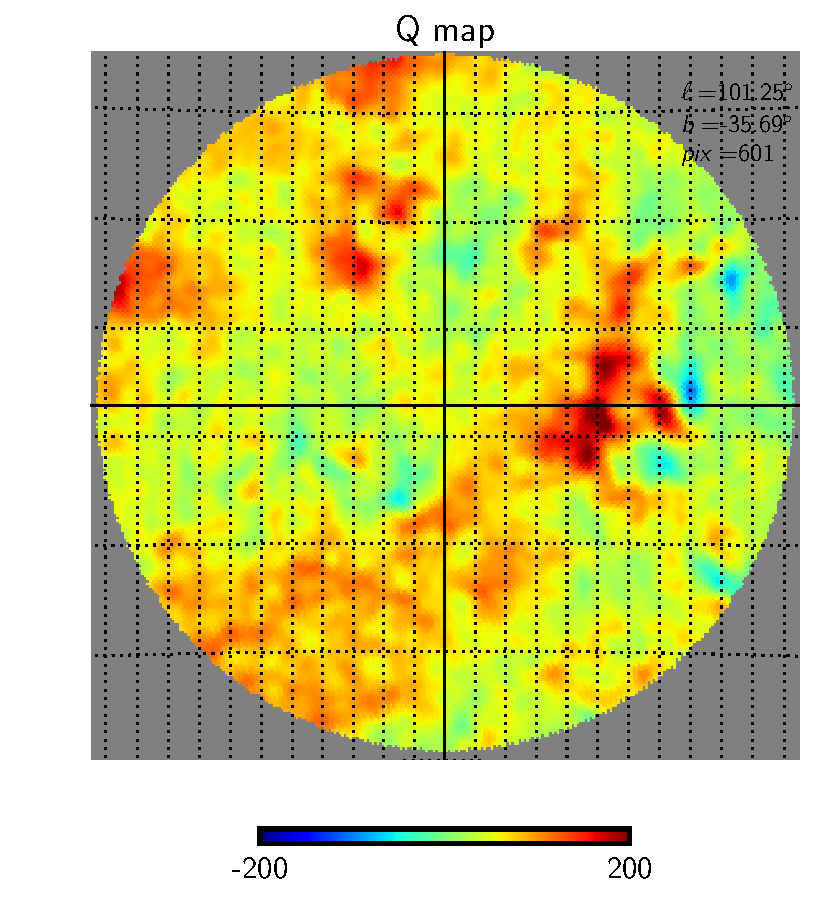
\includegraphics[width=0.1\columnwidth]{bge_scaling0.53/qmap_bge_pix601.pdf}} \hspace{-0.2cm}
\subfigure[U]{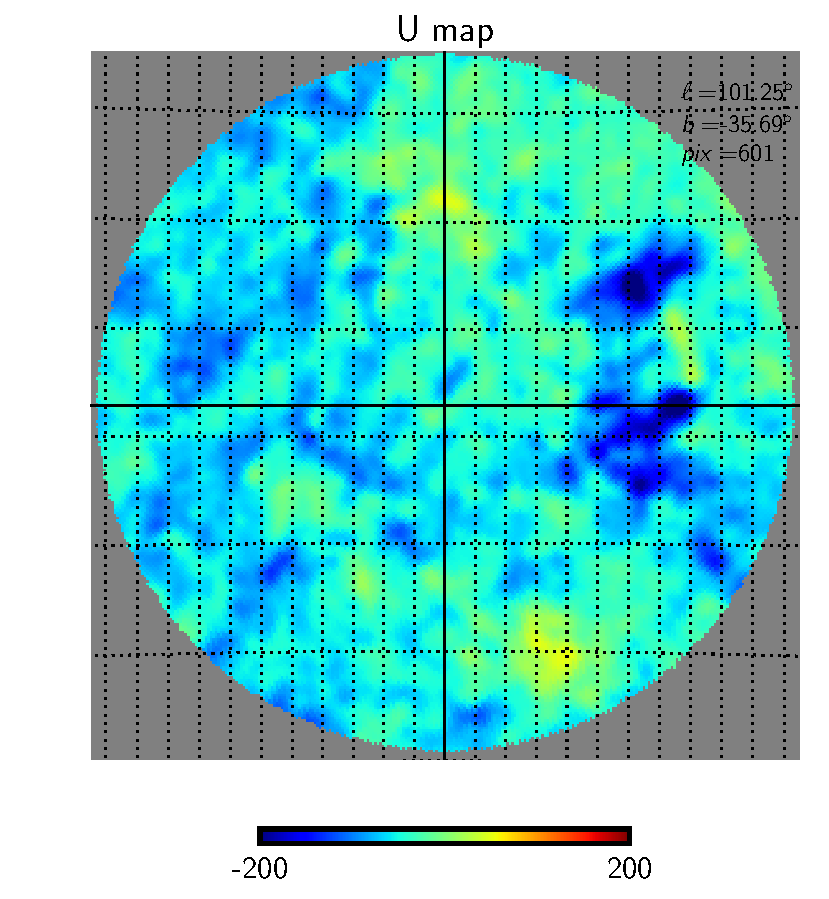
\includegraphics[width=0.1\columnwidth]{bge_scaling0.53/umap_bge_pix601.pdf}} \hspace{-0.2cm}
\subfigure[E(B-V)]{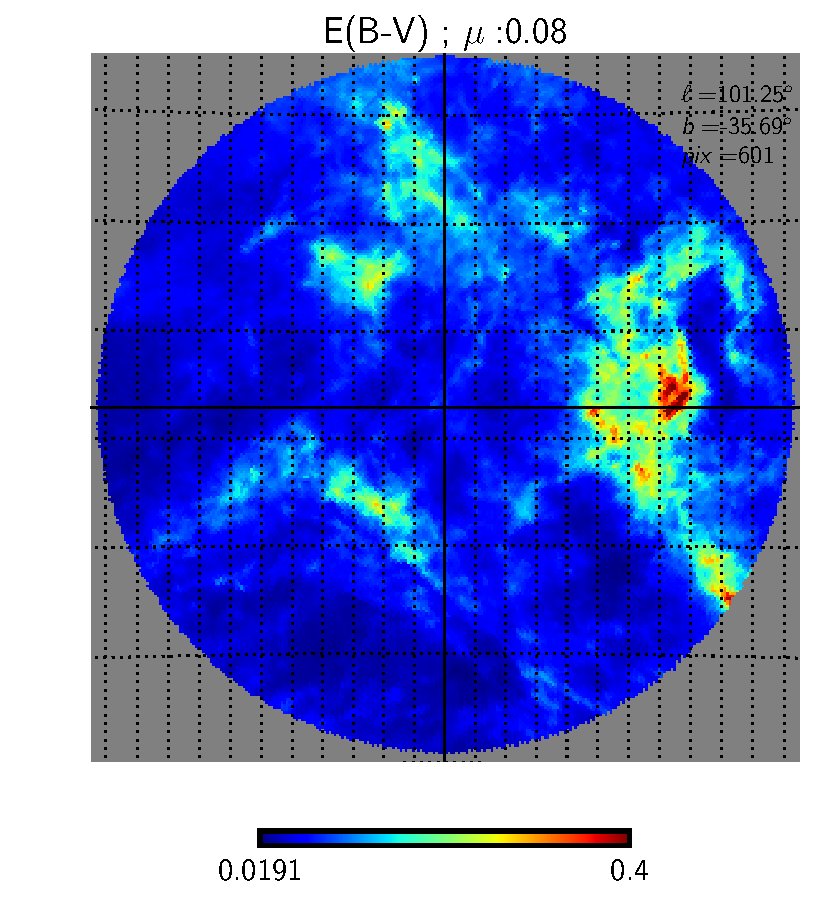
\includegraphics[width=0.1\columnwidth]{bge_scaling0.53/ebv_bge_pix601.pdf}} \hspace{-0.2cm}
\subfigure[E power]{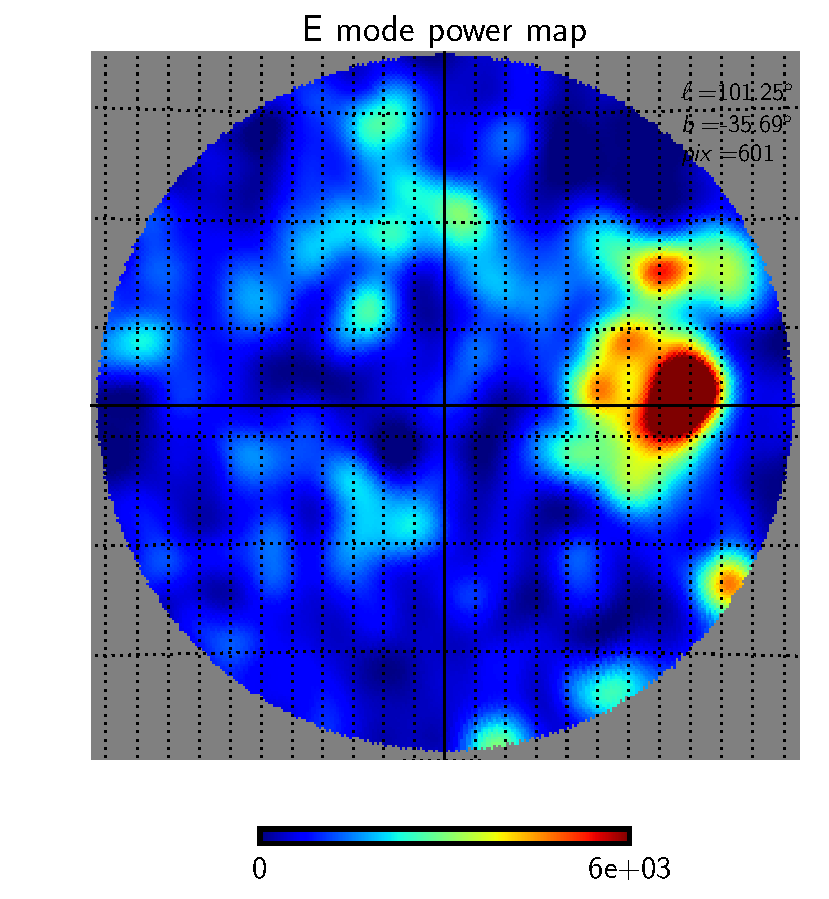
\includegraphics[width=0.1\columnwidth]{bge_scaling0.53/sqemap_bge_pix601.pdf}} \hspace{-0.2cm}
\subfigure[B power]{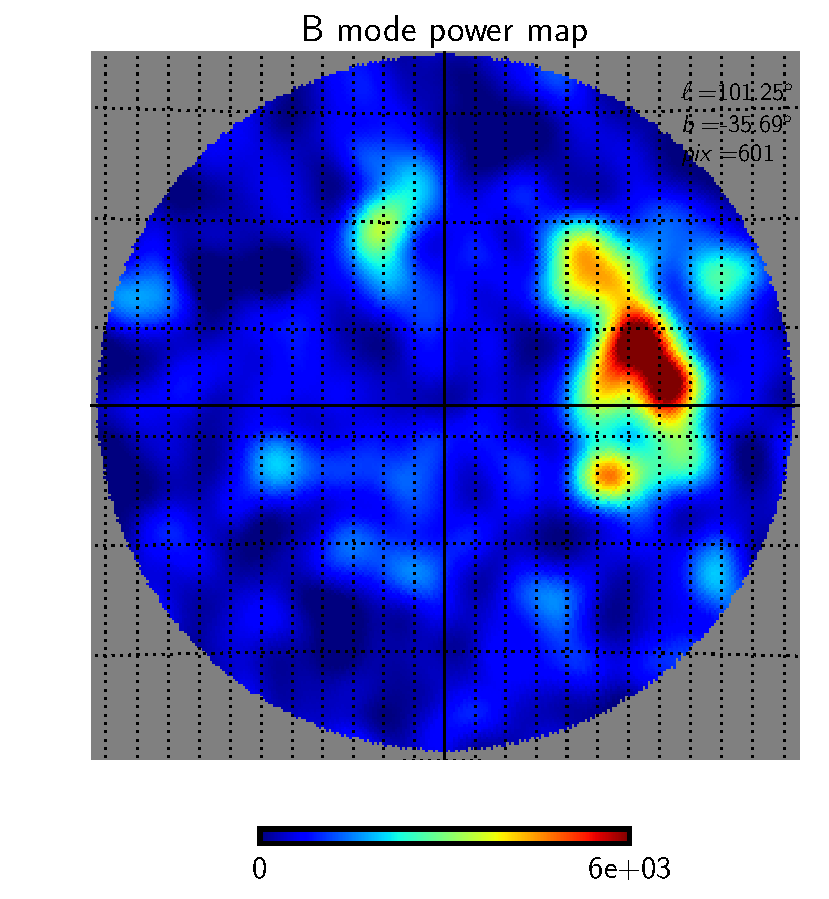
\includegraphics[width=0.1\columnwidth]{bge_scaling0.53/sqbmap_bge_pix601.pdf}} \hspace{-0.2cm}
\subfigure[NH]{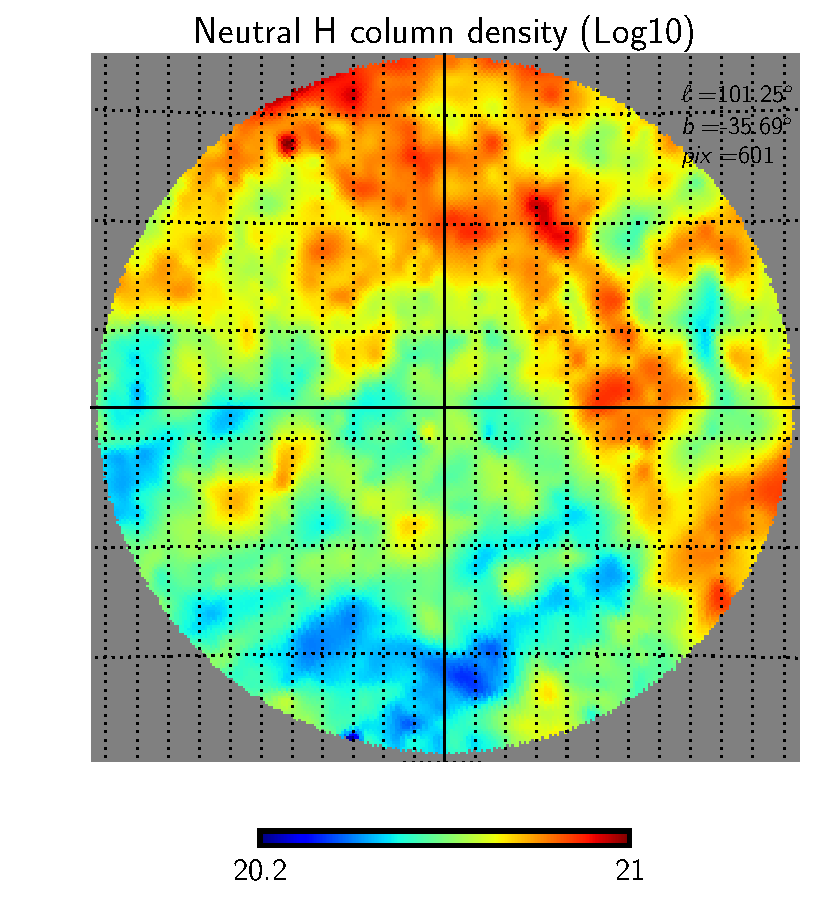
\includegraphics[width=0.1\columnwidth]{bge_scaling0.53/nhcd_bge_pix601.pdf}} \hspace{-0.2cm}
\subfigure[CO]{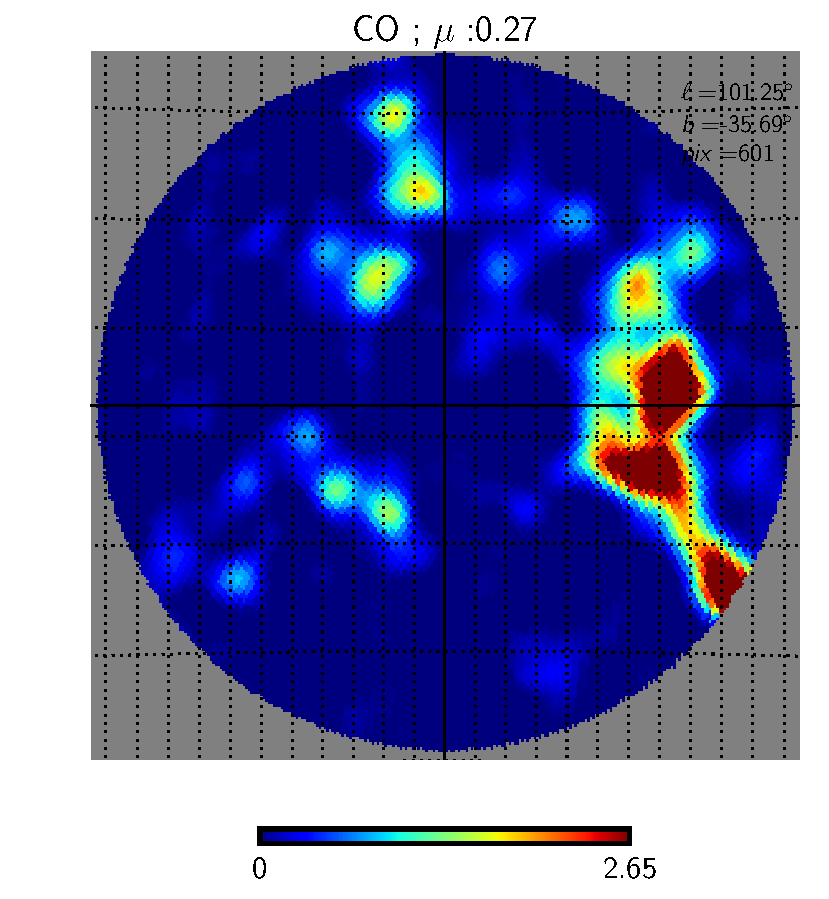
\includegraphics[width=0.1\columnwidth]{bge_scaling0.53/co_bge_pix601.pdf}} \hspace{-0.2cm}
%\subfigure{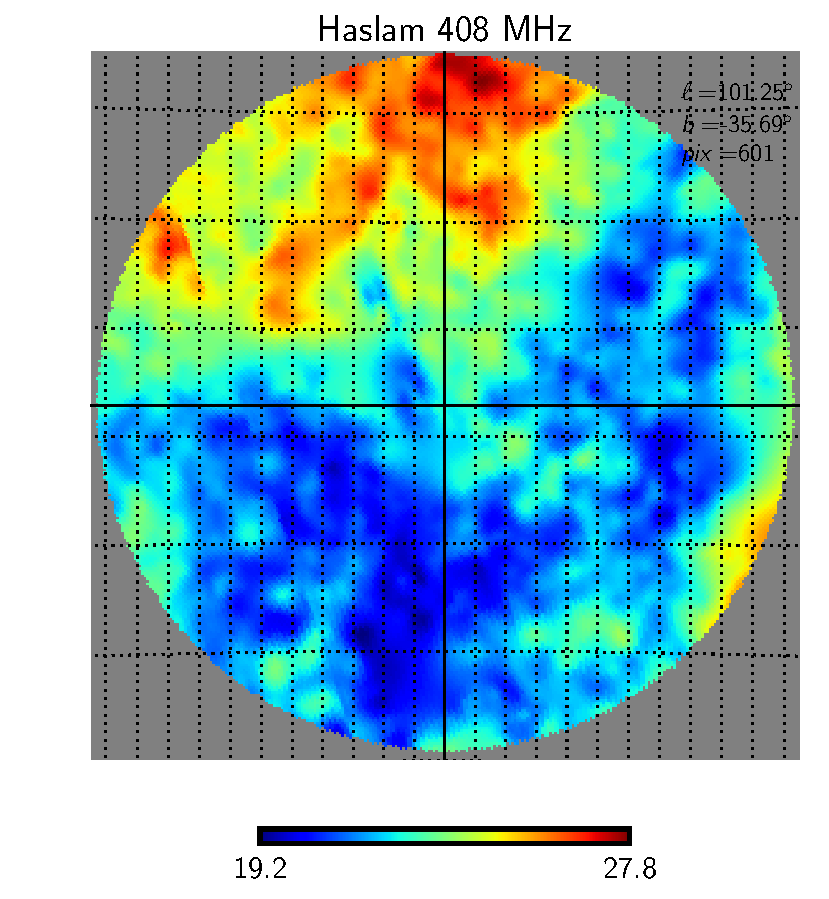
\includegraphics[width=0.1\columnwidth]{bge_scaling0.53/haslam_bge_pix601.pdf}} \hspace{-0.2cm}

\subfigure{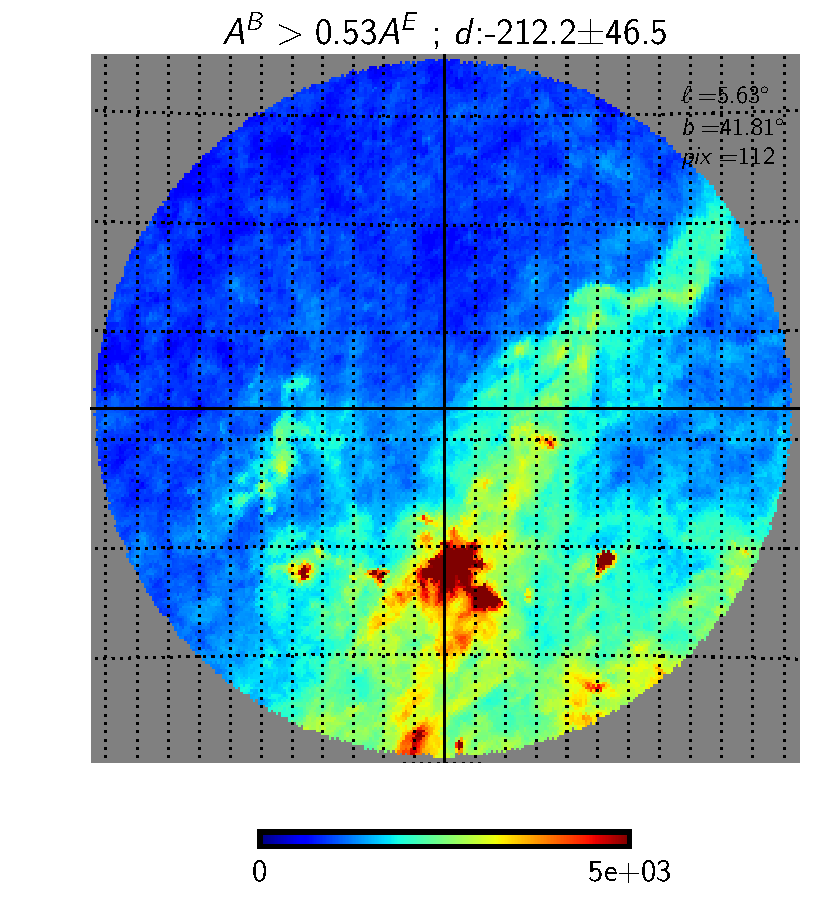
\includegraphics[width=0.1\columnwidth]{bge_scaling0.53/tmap_bge_pix112.pdf}} \hspace{-0.2cm}
\subfigure{\includegraphics[width=0.1\columnwidth]{bge_scaling0.53/emap_bge_pix112.pdf}} \hspace{-0.2cm}
\subfigure{\includegraphics[width=0.1\columnwidth]{bge_scaling0.53/bmap_bge_pix112.pdf}} \hspace{-0.2cm}
\subfigure{\includegraphics[width=0.1\columnwidth]{bge_scaling0.53/qmap_bge_pix112.pdf}} \hspace{-0.2cm}
\subfigure{\includegraphics[width=0.1\columnwidth]{bge_scaling0.53/umap_bge_pix112.pdf}} \hspace{-0.2cm}
\subfigure{\includegraphics[width=0.1\columnwidth]{bge_scaling0.53/ebv_bge_pix112.pdf}} \hspace{-0.2cm}
\subfigure{\includegraphics[width=0.1\columnwidth]{bge_scaling0.53/sqemap_bge_pix112.pdf}} \hspace{-0.2cm}
\subfigure{\includegraphics[width=0.1\columnwidth]{bge_scaling0.53/sqbmap_bge_pix112.pdf}} \hspace{-0.2cm}
\subfigure{\includegraphics[width=0.1\columnwidth]{bge_scaling0.53/nhcd_bge_pix112.pdf}} \hspace{-0.2cm}
\subfigure{\includegraphics[width=0.1\columnwidth]{bge_scaling0.53/co_bge_pix112.pdf}} \hspace{-0.2cm}
%\subfigure{\includegraphics[width=0.1\columnwidth]{bge_scaling0.53/haslam_bge_pix112.pdf}} \hspace{-0.2cm}
%\end{figure}
%\begin{figure}[!h]
\subfigure {\includegraphics[width=0.1\columnwidth]{bge_scaling0.53/tmap_bge_pix691.pdf}} \hspace{-0.2cm}
\subfigure{\includegraphics[width=0.1\columnwidth]{bge_scaling0.53/emap_bge_pix691.pdf}} \hspace{-0.2cm}
\subfigure{\includegraphics[width=0.1\columnwidth]{bge_scaling0.53/bmap_bge_pix691.pdf}} \hspace{-0.2cm}
\subfigure{\includegraphics[width=0.1\columnwidth]{bge_scaling0.53/qmap_bge_pix691.pdf}} \hspace{-0.2cm}
\subfigure{\includegraphics[width=0.1\columnwidth]{bge_scaling0.53/umap_bge_pix691.pdf}} \hspace{-0.2cm}
\subfigure{\includegraphics[width=0.1\columnwidth]{bge_scaling0.53/ebv_bge_pix691.pdf}} \hspace{-0.2cm}
\subfigure{\includegraphics[width=0.1\columnwidth]{bge_scaling0.53/sqemap_bge_pix691.pdf}} \hspace{-0.2cm}
\subfigure{\includegraphics[width=0.1\columnwidth]{bge_scaling0.53/sqbmap_bge_pix691.pdf}} \hspace{-0.2cm}
\subfigure{\includegraphics[width=0.1\columnwidth]{bge_scaling0.53/nhcd_bge_pix691.pdf}} \hspace{-0.2cm}
\subfigure{\includegraphics[width=0.1\columnwidth]{bge_scaling0.53/co_bge_pix691.pdf}} \hspace{-0.2cm}
%\subfigure{\includegraphics[width=0.1\columnwidth]{bge_scaling0.53/haslam_bge_pix691.pdf}} \hspace{-0.2cm}

\subfigure {\includegraphics[width=0.1\columnwidth]{bge_scaling0.53/tmap_bge_pix186.pdf}} \hspace{-0.2cm}
\subfigure{\includegraphics[width=0.1\columnwidth]{bge_scaling0.53/emap_bge_pix186.pdf}} \hspace{-0.2cm}
\subfigure{\includegraphics[width=0.1\columnwidth]{bge_scaling0.53/bmap_bge_pix186.pdf}} \hspace{-0.2cm}
\subfigure{\includegraphics[width=0.1\columnwidth]{bge_scaling0.53/qmap_bge_pix186.pdf}} \hspace{-0.2cm}
\subfigure{\includegraphics[width=0.1\columnwidth]{bge_scaling0.53/umap_bge_pix186.pdf}} \hspace{-0.2cm}
\subfigure{\includegraphics[width=0.1\columnwidth]{bge_scaling0.53/ebv_bge_pix186.pdf}} \hspace{-0.2cm}
\subfigure{\includegraphics[width=0.1\columnwidth]{bge_scaling0.53/sqemap_bge_pix186.pdf}} \hspace{-0.2cm}
\subfigure{\includegraphics[width=0.1\columnwidth]{bge_scaling0.53/sqbmap_bge_pix186.pdf}} \hspace{-0.2cm}
\subfigure{\includegraphics[width=0.1\columnwidth]{bge_scaling0.53/nhcd_bge_pix186.pdf}} \hspace{-0.2cm}
\subfigure{\includegraphics[width=0.1\columnwidth]{bge_scaling0.53/co_bge_pix186.pdf}} \hspace{-0.2cm}
%\subfigure{\includegraphics[width=0.1\columnwidth]{bge_scaling0.53/haslam_bge_pix186.pdf}} \hspace{-0.2cm}
\caption{\color{blue}{$A^{BB}_{sc} > f A^{EE}_{sc}$}}
\end{figure}

\section{Are there regions of the sky where the spectral slope deviates from $\alpha \simeq-2.43$ ? }
Fig.~\ref{fig:eb_slope} depicts the spectral slope for regions of the sky where the polarized dust foreground signal has been measured at a high statistical significance. On these maps we search for pixels where the distance between the measured slope and the global slope is statistically significant: $\frac{|\alpha + 2.43|}{\sigma_{\alpha}} > 3.5$ 
\begin{figure}[!h]
\centering
\subfigure{\includegraphics[width=0.47\columnwidth]{eeslope_snrthr.pdf}}
\subfigure{\includegraphics[width=0.47\columnwidth]{bbslope_snrthr.pdf}}
\caption{These figures depicts the spectral slope of local spectra for E and B mode maps, for regions where the amplitude of the spectra is measured at a high significance.}
\label{fig:eb_slope}
\end{figure}

\begin{figure}[!h]
\centering
\subfigure{\includegraphics[width=0.4\columnwidth]{eebb_slope_scatter.pdf}}\\
\subfigure{\includegraphics[width=0.47\columnwidth]{ee_dev_slope.pdf}}
\subfigure{\includegraphics[width=0.47\columnwidth]{bb_dev_slope.pdf}}
\caption{These figures depicts the spectral slopes  of E and B spectra which are deviant from the global spectral slope of -2.43. The bottom left shows the spatial distribution of regions where the EE spectrum have a deviant slope while the bottom right shows the regions where the BB spectrum have a deviant spectral slope.}
\label{fig:eb_slope_dev}
\end{figure}

We note that most of the regions with a deviant slope are seen to have a shallower spectrum ($\alpha > -2.43$).

\begin{figure}[!h]
\subfigure[T]{\includegraphics[width=0.1\columnwidth]{ebslope_deviant/tmap_sld_pix616.pdf}} \hspace{-0.2cm}
\subfigure[E]{\includegraphics[width=0.1\columnwidth]{ebslope_deviant/emap_sld_pix616.pdf}} \hspace{-0.2cm}
\subfigure[B]{\includegraphics[width=0.1\columnwidth]{ebslope_deviant/bmap_sld_pix616.pdf}} \hspace{-0.2cm}
\subfigure[Q]{\includegraphics[width=0.1\columnwidth]{ebslope_deviant/qmap_sld_pix616.pdf}} \hspace{-0.2cm}
\subfigure[U]{\includegraphics[width=0.1\columnwidth]{ebslope_deviant/umap_sld_pix616.pdf}} \hspace{-0.2cm}
\subfigure[E(B-V)]{\includegraphics[width=0.1\columnwidth]{ebslope_deviant/ebv_sld_pix616.pdf}} \hspace{-0.2cm}
\subfigure[E power]{\includegraphics[width=0.1\columnwidth]{ebslope_deviant/sqemap_sld_pix616.pdf}} \hspace{-0.2cm}
\subfigure[B power]{\includegraphics[width=0.1\columnwidth]{ebslope_deviant/sqbmap_sld_pix616.pdf}} \hspace{-0.2cm}
\subfigure[NH]{\includegraphics[width=0.1\columnwidth]{ebslope_deviant/nhcd_sld_pix616.pdf}} \hspace{-0.2cm}
\subfigure[CO]{\includegraphics[width=0.1\columnwidth]{ebslope_deviant/co_sld_pix616.pdf}} \hspace{-0.2cm}
%\subfigure{\includegraphics[width=0.1\columnwidth]{ebslope_deviant/haslam_sld_pix616.pdf}} \hspace{-0.2cm}
%\end{figure}
%\begin{figure}[!h]
\subfigure {\includegraphics[width=0.1\columnwidth]{ebslope_deviant/tmap_sld_pix553.pdf}} \hspace{-0.2cm}
\subfigure{\includegraphics[width=0.1\columnwidth]{ebslope_deviant/emap_sld_pix553.pdf}} \hspace{-0.2cm}
\subfigure{\includegraphics[width=0.1\columnwidth]{ebslope_deviant/bmap_sld_pix553.pdf}} \hspace{-0.2cm}
\subfigure{\includegraphics[width=0.1\columnwidth]{ebslope_deviant/qmap_sld_pix553.pdf}} \hspace{-0.2cm}
\subfigure{\includegraphics[width=0.1\columnwidth]{ebslope_deviant/umap_sld_pix553.pdf}} \hspace{-0.2cm}
\subfigure{\includegraphics[width=0.1\columnwidth]{ebslope_deviant/ebv_sld_pix553.pdf}} \hspace{-0.2cm}
\subfigure{\includegraphics[width=0.1\columnwidth]{ebslope_deviant/sqemap_sld_pix553.pdf}} \hspace{-0.2cm}
\subfigure{\includegraphics[width=0.1\columnwidth]{ebslope_deviant/sqbmap_sld_pix553.pdf}} \hspace{-0.2cm}
\subfigure{\includegraphics[width=0.1\columnwidth]{ebslope_deviant/nhcd_sld_pix553.pdf}} \hspace{-0.2cm}
\subfigure{\includegraphics[width=0.1\columnwidth]{ebslope_deviant/co_sld_pix553.pdf}} \hspace{-0.2cm}
%\subfigure{\includegraphics[width=0.1\columnwidth]{ebslope_deviant/haslam_sld_pix553.pdf}} \hspace{-0.2cm}

\subfigure {\includegraphics[width=0.1\columnwidth]{ebslope_deviant/tmap_sld_pix584.pdf}} \hspace{-0.2cm}
\subfigure{\includegraphics[width=0.1\columnwidth]{ebslope_deviant/emap_sld_pix584.pdf}} \hspace{-0.2cm}
\subfigure{\includegraphics[width=0.1\columnwidth]{ebslope_deviant/bmap_sld_pix584.pdf}} \hspace{-0.2cm}
\subfigure{\includegraphics[width=0.1\columnwidth]{ebslope_deviant/qmap_sld_pix584.pdf}} \hspace{-0.2cm}
\subfigure{\includegraphics[width=0.1\columnwidth]{ebslope_deviant/umap_sld_pix584.pdf}} \hspace{-0.2cm}
\subfigure{\includegraphics[width=0.1\columnwidth]{ebslope_deviant/ebv_sld_pix584.pdf}} \hspace{-0.2cm}
\subfigure{\includegraphics[width=0.1\columnwidth]{ebslope_deviant/sqemap_sld_pix584.pdf}} \hspace{-0.2cm}
\subfigure{\includegraphics[width=0.1\columnwidth]{ebslope_deviant/sqbmap_sld_pix584.pdf}} \hspace{-0.2cm}
\subfigure{\includegraphics[width=0.1\columnwidth]{ebslope_deviant/nhcd_sld_pix584.pdf}} \hspace{-0.2cm}
\subfigure{\includegraphics[width=0.1\columnwidth]{ebslope_deviant/co_sld_pix584.pdf}} \hspace{-0.2cm}
%\subfigure{\includegraphics[width=0.1\columnwidth]{ebslope_deviant/haslam_sld_pix584.pdf}} \hspace{-0.2cm}

\subfigure {\includegraphics[width=0.1\columnwidth]{ebslope_deviant/tmap_sld_pix648.pdf}} \hspace{-0.2cm}
\subfigure{\includegraphics[width=0.1\columnwidth]{ebslope_deviant/emap_sld_pix648.pdf}} \hspace{-0.2cm}
\subfigure{\includegraphics[width=0.1\columnwidth]{ebslope_deviant/bmap_sld_pix648.pdf}} \hspace{-0.2cm}
\subfigure{\includegraphics[width=0.1\columnwidth]{ebslope_deviant/qmap_sld_pix648.pdf}} \hspace{-0.2cm}
\subfigure{\includegraphics[width=0.1\columnwidth]{ebslope_deviant/umap_sld_pix648.pdf}} \hspace{-0.2cm}
\subfigure{\includegraphics[width=0.1\columnwidth]{ebslope_deviant/ebv_sld_pix648.pdf}} \hspace{-0.2cm}
\subfigure{\includegraphics[width=0.1\columnwidth]{ebslope_deviant/sqemap_sld_pix648.pdf}} \hspace{-0.2cm}
\subfigure{\includegraphics[width=0.1\columnwidth]{ebslope_deviant/sqbmap_sld_pix648.pdf}} \hspace{-0.2cm}
\subfigure{\includegraphics[width=0.1\columnwidth]{ebslope_deviant/nhcd_sld_pix648.pdf}} \hspace{-0.2cm}
\subfigure{\includegraphics[width=0.1\columnwidth]{ebslope_deviant/co_sld_pix648.pdf}} \hspace{-0.2cm}
%\subfigure{\includegraphics[width=0.1\columnwidth]{ebslope_deviant/haslam_sld_pix648.pdf}} \hspace{-0.2cm}
\caption{\color{black}{$\alpha_{EE} ~ \& ~ \alpha_{BB} \neq -2.43$}}
\end{figure}


\begin{figure}[!h]
\subfigure[T]{\includegraphics[width=0.1\columnwidth]{ebslope_deviant/tmap_sld_pix77.pdf}} \hspace{-0.2cm}
\subfigure[E]{\includegraphics[width=0.1\columnwidth]{ebslope_deviant/emap_sld_pix77.pdf}} \hspace{-0.2cm}
\subfigure[B]{\includegraphics[width=0.1\columnwidth]{ebslope_deviant/bmap_sld_pix77.pdf}} \hspace{-0.2cm}
\subfigure[Q]{\includegraphics[width=0.1\columnwidth]{ebslope_deviant/qmap_sld_pix77.pdf}} \hspace{-0.2cm}
\subfigure[U]{\includegraphics[width=0.1\columnwidth]{ebslope_deviant/umap_sld_pix77.pdf}} \hspace{-0.2cm}
\subfigure[E(B-V)]{\includegraphics[width=0.1\columnwidth]{ebslope_deviant/ebv_sld_pix77.pdf}} \hspace{-0.2cm}
\subfigure[E power]{\includegraphics[width=0.1\columnwidth]{ebslope_deviant/sqemap_sld_pix77.pdf}} \hspace{-0.2cm}
\subfigure[B power]{\includegraphics[width=0.1\columnwidth]{ebslope_deviant/sqbmap_sld_pix77.pdf}} \hspace{-0.2cm}
\subfigure[NH]{\includegraphics[width=0.1\columnwidth]{ebslope_deviant/nhcd_sld_pix77.pdf}} \hspace{-0.2cm}
\subfigure[CO]{\includegraphics[width=0.1\columnwidth]{ebslope_deviant/co_sld_pix77.pdf}} \hspace{-0.2cm}
%\subfigure{\includegraphics[width=0.1\columnwidth]{ebslope_deviant/haslam_sld_pix77.pdf}} \hspace{-0.2cm}
%\end{figure}
%\begin{figure}[!h]
\subfigure {\includegraphics[width=0.1\columnwidth]{ebslope_deviant/tmap_sld_pix79.pdf}} \hspace{-0.2cm}
\subfigure{\includegraphics[width=0.1\columnwidth]{ebslope_deviant/emap_sld_pix79.pdf}} \hspace{-0.2cm}
\subfigure{\includegraphics[width=0.1\columnwidth]{ebslope_deviant/bmap_sld_pix79.pdf}} \hspace{-0.2cm}
\subfigure{\includegraphics[width=0.1\columnwidth]{ebslope_deviant/qmap_sld_pix79.pdf}} \hspace{-0.2cm}
\subfigure{\includegraphics[width=0.1\columnwidth]{ebslope_deviant/umap_sld_pix79.pdf}} \hspace{-0.2cm}
\subfigure{\includegraphics[width=0.1\columnwidth]{ebslope_deviant/ebv_sld_pix79.pdf}} \hspace{-0.2cm}
\subfigure{\includegraphics[width=0.1\columnwidth]{ebslope_deviant/sqemap_sld_pix79.pdf}} \hspace{-0.2cm}
\subfigure{\includegraphics[width=0.1\columnwidth]{ebslope_deviant/sqbmap_sld_pix79.pdf}} \hspace{-0.2cm}
\subfigure{\includegraphics[width=0.1\columnwidth]{ebslope_deviant/nhcd_sld_pix79.pdf}} \hspace{-0.2cm}
\subfigure{\includegraphics[width=0.1\columnwidth]{ebslope_deviant/co_sld_pix79.pdf}} \hspace{-0.2cm}
%\subfigure{\includegraphics[width=0.1\columnwidth]{ebslope_deviant/haslam_sld_pix79.pdf}} \hspace{-0.2cm}
\caption{\color{red}{$\alpha_{EE} \neq -2.43$}}
\end{figure}

\begin{figure}[!h]
\subfigure[T]{\includegraphics[width=0.1\columnwidth]{ebslope_deviant/tmap_sld_pix2.pdf}} \hspace{-0.2cm}
\subfigure[E]{\includegraphics[width=0.1\columnwidth]{ebslope_deviant/emap_sld_pix2.pdf}} \hspace{-0.2cm}
\subfigure[B]{\includegraphics[width=0.1\columnwidth]{ebslope_deviant/bmap_sld_pix2.pdf}} \hspace{-0.2cm}
\subfigure[Q]{\includegraphics[width=0.1\columnwidth]{ebslope_deviant/qmap_sld_pix2.pdf}} \hspace{-0.2cm}
\subfigure[U]{\includegraphics[width=0.1\columnwidth]{ebslope_deviant/umap_sld_pix2.pdf}} \hspace{-0.2cm}
\subfigure[E(B-V)]{\includegraphics[width=0.1\columnwidth]{ebslope_deviant/ebv_sld_pix2.pdf}} \hspace{-0.2cm}
\subfigure[E power]{\includegraphics[width=0.1\columnwidth]{ebslope_deviant/sqemap_sld_pix2.pdf}} \hspace{-0.2cm}
\subfigure[B power]{\includegraphics[width=0.1\columnwidth]{ebslope_deviant/sqbmap_sld_pix2.pdf}} \hspace{-0.2cm}
\subfigure[NH]{\includegraphics[width=0.1\columnwidth]{ebslope_deviant/nhcd_sld_pix2.pdf}} \hspace{-0.2cm}
\subfigure[CO]{\includegraphics[width=0.1\columnwidth]{ebslope_deviant/co_sld_pix2.pdf}} \hspace{-0.2cm}
%\subfigure{\includegraphics[width=0.1\columnwidth]{ebslope_deviant/haslam_sld_pix2.pdf}} \hspace{-0.2cm}
%\end{figure}
%\begin{figure}[!h]
\subfigure {\includegraphics[width=0.1\columnwidth]{ebslope_deviant/tmap_sld_pix612.pdf}} \hspace{-0.2cm}
\subfigure{\includegraphics[width=0.1\columnwidth]{ebslope_deviant/emap_sld_pix612.pdf}} \hspace{-0.2cm}
\subfigure{\includegraphics[width=0.1\columnwidth]{ebslope_deviant/bmap_sld_pix612.pdf}} \hspace{-0.2cm}
\subfigure{\includegraphics[width=0.1\columnwidth]{ebslope_deviant/qmap_sld_pix612.pdf}} \hspace{-0.2cm}
\subfigure{\includegraphics[width=0.1\columnwidth]{ebslope_deviant/umap_sld_pix612.pdf}} \hspace{-0.2cm}
\subfigure{\includegraphics[width=0.1\columnwidth]{ebslope_deviant/ebv_sld_pix612.pdf}} \hspace{-0.2cm}
\subfigure{\includegraphics[width=0.1\columnwidth]{ebslope_deviant/sqemap_sld_pix612.pdf}} \hspace{-0.2cm}
\subfigure{\includegraphics[width=0.1\columnwidth]{ebslope_deviant/sqbmap_sld_pix612.pdf}} \hspace{-0.2cm}
\subfigure{\includegraphics[width=0.1\columnwidth]{ebslope_deviant/nhcd_sld_pix612.pdf}} \hspace{-0.2cm}
\subfigure{\includegraphics[width=0.1\columnwidth]{ebslope_deviant/co_sld_pix612.pdf}} \hspace{-0.2cm}
%\subfigure{\includegraphics[width=0.1\columnwidth]{ebslope_deviant/haslam_sld_pix612.pdf}} \hspace{-0.2cm}
\caption{\color{blue}{$\alpha_{BB} \neq -2.43$}}
\end{figure}

\section{Summary}
\begin{itemize}
\item We have identified a set of regions where the E and B spectra don't follow the spectral amplitude scaling relation and regions where the spectral slope is deviant from the slopes inferred from the global analysis.
\item Regions where the slope is deviant from the global slope do not coincide with regions where the spectral amplitude scaling relation is anomalous.
\item We find at least one region of the sky where both E and B spectra have a shallower spectral slope $\alpha \sim -1.5$ as compared to the global spectral slope of $\alpha=-2.43$.
\item Often neighboring pixels are seen to show similar trends, since the mask uncovers the same regions of the sky for these neighboring pixel centers.
\end{itemize}


\begin{figure}[!h]
\centering
\subfigure{\includegraphics[width=0.3\columnwidth]{t353_moll.pdf}}
\subfigure{\includegraphics[width=0.3\columnwidth]{e353_moll.pdf}}
\subfigure{\includegraphics[width=0.3\columnwidth]{b353_moll.pdf}}
\subfigure{\includegraphics[width=0.3\columnwidth]{te353_moll.pdf}}
\subfigure{\includegraphics[width=0.3\columnwidth]{tb353_moll.pdf}}
\caption{}
\end{figure}

\appendix
\section{Supplementary plots}
\begin{figure}[!h]
\centering
\subfigure{\includegraphics[width=0.47\columnwidth]{e353_sq.pdf}}
\subfigure{\includegraphics[width=0.47\columnwidth]{b353_sq.pdf}}
\subfigure{\includegraphics[width=0.47\columnwidth]{b353ce353.pdf}}
\subfigure{\includegraphics[width=0.47\columnwidth]{tpow.pdf}}
\caption{}
\end{figure}

\begin{figure}[!h]
\subfigure{\includegraphics[width=0.5\columnwidth]{E-pol_amplitude_vs_dust_intensity.pdf}}
\subfigure{\includegraphics[width=0.5\columnwidth]{B-pol_amplitude_vs_dust_intensity.pdf}}
\caption{}
\end{figure}

\begin{figure}[!h]
\centering
\subfigure{\includegraphics[width=0.47\columnwidth]{epol_slope_vs_theta.pdf}}
\subfigure{\includegraphics[width=0.47\columnwidth]{bpol_slope_vs_theta.pdf}}
\subfigure{\includegraphics[width=0.47\columnwidth]{ebamp_ratio_vs_theta.pdf}}
\subfigure{\includegraphics[width=0.47\columnwidth]{ebamp-ratio_vs_slope_ratio.pdf}}
\caption{}
\end{figure}

\end{document}
